\documentclass[suppldata]{interact}

\usepackage{epstopdf}% To incorporate .eps illustrations using PDFLaTeX, etc.
\usepackage[caption=false]{subfig}% Support for small, `sub' figures and tables

%\usepackage[nolists,tablesfirst]{endfloat}% To `separate' figures tables from text if required
%\usepackage[doublespacing]{setspace}% To produce a `double spaced' document if required
%\setlength\parindent{24pt}% To increase paragraph indentation when line spacing is doubled

\usepackage{soul}
\usepackage{amsmath,amssymb} 
\usepackage[natbibapa,nodoi]{apacite}
\usepackage{multicol}
\setlength\bibhang{12pt}
\renewcommand\bibliographytypesize{\fontsize{10}{12}\selectfont}
\theoremstyle{plain}
\newtheorem{theorem}{Theorem}[section]
\newtheorem{lemma}[theorem]{Lemma}
\newtheorem{corollary}[theorem]{Corollary}
\newtheorem{proposition}[theorem]{Proposition}

\theoremstyle{definition}
\newtheorem{definition}[theorem]{Definition}
\newtheorem{example}[theorem]{Example}

\theoremstyle{remark}
\newtheorem{remark}{Remark}
\newtheorem{notation}{Notation}

\usepackage[pdftex,colorlinks=true,urlcolor=blue,citecolor=black,anchorcolor=black,linkcolor=black]{hyperref}
\usepackage{xcolor}
\usepackage{algorithm} 
\usepackage{algorithmic} 
\renewcommand{\algorithmicrequire}{ \textbf{Input:}}
\usepackage{soul}
\setlength{\marginparwidth}{2cm}
\usepackage{todonotes}
\usepackage{lscape}

%%%%%%%%%%%%%%		Breakable Algorithm		%%%%%%%%%%%%%%%%%%%%%%
\makeatletter
\newenvironment{breakablealgorithm}
{% \begin{breakablealgorithm}
	\begin{center}
		\refstepcounter{algorithm}% New algorithm
		\hrule height.8pt depth0pt \kern2pt% \@fs@pre for \@fs@ruled
		\renewcommand{\caption}[2][\relax]{% Make a new \caption
			{\raggedright\textbf{\ALG@name~\thealgorithm} ##2\par}%
			\ifx\relax##1\relax % #1 is \relax
			\addcontentsline{loa}{algorithm}{\protect\numberline{\thealgorithm}##2}%
			\else % #1 is not \relax
			\addcontentsline{loa}{algorithm}{\protect\numberline{\thealgorithm}##1}%
			\fi
			\kern2pt\hrule\kern2pt
		}
	}{% \end{breakablealgorithm}
		\kern2pt\hrule\relax% \@fs@post for \@fs@ruled
	\end{center}
}
\makeatother
%%%%%%%%%%%%%%		Breakable Algorithm		%%%%%%%%%%%%%%%%%%%%%%

%\usepackage[affil-it]{authblk}
%\renewcommand\Authfont{\fontsize{10}{14.4}\selectfont}
%\renewcommand\Affilfont{\fontsize{8}{10.8}\itshape}

\begin{document}

\author{\name{Mengyi Zhang\textsuperscript{a}\thanks{CONTACT Mengyi Zhang. Email: mengyi.zhang@polimi.it}, Arianna Alfieri\textsuperscript{b}, Andrea Matta\textsuperscript{a}}
\medskip
\affil{\small \textsuperscript{a} Department of Mechanical Engineering, Politecnico di Milano, via La Masa 1, 20156 Milano, Italy}
\affil{\small \textsuperscript{b} Department of Management and Industrial Engineering, Politecnico di Torino, Corso Duca degli Abruzzi 24, 10129 Turin, Italy}}


\title{\Large From black box to white box: automated generation of mathematical programming representation for discrete event simulation models}

\maketitle

\bigskip
\begin{abstract}
This work proposes a mathematical programming (MP) representation of discrete event simulation of timed Petri nets (TPN). Currently, MP techniques are not widely applied to optimizing discrete event systems, however, this work builds a connection between the two fruitful research fields. In the MP formalism, the decision variables are composed of the transition firing time and the markings, while the constraints represents the state transition logic and temporal sequences among events. The MP model and a simulation run of the TPN are totally equivalent, which is validated with several cases. Using a TPN model as input, the MP model can be routinely and conveniently generated.


%It is a new formalism of discrete event systems. The MPR-DES is the foundation of developing white-box simulation optimization algorithms. The decision variables of the MPR are the transition firing times and the markings, and the constraints represent the transition firings. The equivalence of the solution of the proposed mathematical programming model and the simulation run using the same sample paths is validated with several cases. The MPR generation has been coded in an automatic procedure that only requires the user to input the timed Petri net model.
\end{abstract}

\begin{keywords}
discrete event simulation, mathematical programming, timed Petri net
\end{keywords}


\section{Introduction}

Discrete event systems has wide application in manufacturing and service applications. Even though many theoretical and analytical studies on discrete event dynamic systems have been developed, performance of real systems sometimes can only be evaluating with discrete event simulation (DES) due to system complexity. Hence, simulation--optimization algorithms are widely used when performance evaluation must be coupled with optimization, i.e., when the best system configuration, according to some criteria, has to be found meanwhile guaranteeing a given value of some performance measure.  


Most of the simulation--optimization studies consider DES as a \textit{black--box} function. Under the black--box setting, simulation module and optimization module are decoupled, except that simulation module needs to provide the performance measures of certain solutions when the optimization module queries. with quite limited information from simulation, the optimization module must have many trials, so the black--box procedure can be computationally inefficient.


A promising direction to improve the inefficiency of black-box procedure is to merge the system dynamics into optimization, i.e., considering DES as white-box and modeling system dynamics as part of mathematical programming (MP) models. Several works can be found in literature. An MP model was proposed to minimize the makespan of single-server manufacturing systems in \cite{di2020makespan}. The buffer allocation problem in multi-stage production flow lines with blocking is formulated as MP and solved in \cite{matta2008simulation}, \cite{weiss2015buffer} and \cite{alfieri2020time}. The optimization of systems with complex blocking mechanisms, for instance extended kanban, is addressed in \cite{pedrielli2015integrated} with MP techniques. With MP techniques, such as decomposition or linear approximation, solving the MP models can be rather efficient than black-box algorithms and the optimality is also enhanced (\cite{weiss2015buffer}, \cite{alfieri2020time}). 


However, white-box simulation optimization approaches are not as widely-applied as block-box ones. The reason is that developing a white-box algorithm requires one to master both discrete event dynamic systems, its simulation and mathematical programming, but those disciplines are not tightly connected. The above-mentioned works all addresses the optimization of systems with specific assumptions, and there is a lack of generalization to extend the approaches into other problems. To fill this gap, this work proposes an approach to translating the simulation of general timed Petri net (TPN) into MP models.


In literature, a few works address the same problem as this one, i.e.,  translating the behavior of general discrete event dynamic systems into MP. \cite{bemporad1999control} proposed a mixed integer programming modeling framework for hybrid systems, whose states are mixed integer, in discrete time. Differently, this work deals with continuous--time discrete--state systems. \cite{chan2008optimization} proposed a modeling framework to translate a DES model into an MPR model in a general sense. Their modeling framework is based on the Event Relationship Graph (ERG) of the system dynamics. However, the ERG is not as commonly-used as TPN, so people would very probably prefer to have a TPN-based approach than ERG-based. 


The benefits of using MP model to present discrete event systems are many. As already mentioned above, when coupled with optimization, the MP-based algorithms can be faster and gain better solution than black--box optimization algorithms. Furthermore, black--box approaches have limited capability is solving constrained optimization problems, but MP-based approaches can easily deal with them \cite{zhang2020models}. Thirdly, the vast theoretical and methodological results developed in the MP field can be introduced into the study of DEVS through simulation. For instance, using sensitivity analysis of MP models, DES can be a gradient estimation tool, as suggested in \cite{chan2008optimization}. In fact, we do not proposed to totally replace simulation with MP, but to enrich the toolbox for analyzing and optimizing DEVS. Finally, the application of MP models of DEVS is not limited to optimization. \cite{basile2012k} proposed the sufficient and necessary condition of K-diagnosability of TPN based on MP modeling. 


The major concern about the application of MP is the computational complexity. Solving MP models can be time-consuming or even unbearable. However, many approaches from optimization community are available to improve the efficiency. Linear programming approximation (\cite{alfieri2012mathematical}), Benders decomposition (\cite{weiss2015buffer}), row-column generation (\cite{alfieri2020time}), have been studied to solve optimization problems in reality based-on MP model of DEVS.


The contributions of this work is to propose the first framework translating general TPN into MP models. The translation procedure can be conveniently implemented in general purpose programming languages. This work lays a foundation of developing MP-based algorithm for analyzing and optimizing general TPN, based on the vast literature in MP filed. 
%The proposed MP models can also be easily transformed into an MPR for optimizing the design parameters of the DES, which are common optimization problems in operations management field.  


The rest of the paper is organized as follows. Section \ref{sec:sim} briefly introduce the TPN and its simulation algorithm. Section \ref{sec:TPN_MPR} describes the generation of the MPR of a TPN model. Section XXX shows several examples of application and validation of the equivalence of simulation and the MP. Discussion and conclusion are reported in Section XXX and XXX, respectively.



%alternating simulation and optimization procedures, thus, possibly leading to computational inefficiency if the number of iterations and/or the computation time per iteration increases too much. 

% On the contrary, a minority of the simulation--optimization literature explores the structure of the DES models, and such approaches are referred to as \textit{white--box} simulation--optimization. 



%The benefit of white--box simulation--optimization is the saving of simulation budget or computation time since the optimization procedure is guided by the information contained in the structure of the DES model (\cite{zhang2020sample}). However, the barrier to the use of white--box simulation--optimization is modeling DES as white box, so that it eventually favors optimization. 


%The benefit of developing an MPR might be not obvious (especially when there is already a DES model) due to the extremely high complexity of solving it. 
%One may be confused about the motivation of this work, i.e., why one wants the MPR when he/she has already a simulation model at hand, since the complexity of solving mathematical programming is usually high. 
%However, this work does not suggest solving the MPR directly with state-of-the-art optimizers. Instead, the optimal solution of the MPR can be obtained from a simulation run. The added value of the MPR is that the structure of the DES can be explored. With the vast theoretical and methodological results developed in the mathematical programming (MP) field, for instance sensitivity analysis as suggested by \cite{chan2008optimization}, the MPR of a simulation model favors the optimal design and control of the discrete event systems. 

%This work proposes a procedure to establish a white--box simulation model, which is an equivalent Mathematical Programming Representation (MPR) model, based on the well-known event--scheduling logic (\cite{law2014simulation}) applied to timed Petri net (TPN). %for  
%The procedure is applicable to certain types of DES models, and the assumptions that the DES model should satisfy are also presented in this work.
%Specifically, the modeling procedure, the assumptions which the DES model has to satisfy so that it can be applied and some examples are discussed. 

%In this work, we present how to establish an equivalent Mathematical Programming Representation (MPR) of Discrete Event Simulation (DES). The MPR depicts the dynamics of an event-scheduling approach of simulation modeling with a certain sample path. To develop the MPR, state variables, events, initial state, termination condition and the samples of the random variate should be provided. All requirement is also essential each time an event-scheduling algorithm is programmed. Furthermore, the proposed approach is quite routined. Thus, no extra knowledge or skills are required when one has the event-scheduling simulation implementation and wants to apply our approach. Besides the modeling approach, we provide the conditions to check before applying our approach, and discuss what the modifications can be done when some conditions are violated. Some examples are also given.

%Considering the literature on simulation--optimization, 
%\cite{chan2008optimization} proposed a modeling framework to translate a DES model into an MPR model in a general sense. Their modeling framework is based on the Event Relationship Graph (ERG) of the system dynamics. To derive the MPR, % model, 
%an ERG of the DES must be constructed and expanded to an elementary ERG (EERG) model, and a procedure can be applied to translate the EERG model into an MPR. %model. 
%However, this procedure has some limitations. First, deriving an ERG is not an easy task, and the user must pay quite much attention to detect all the event relationships and complete the triggering conditions between each pair of related events. %That 
%The difficulty of developing ERG limits the wide spread of this procedure. Second, the modeling procedure is case--by--case depending on the event relationships, which means that the user must analyze the event relationships one by one and identify which type of modeling, including the variables and constraints, he/she should apply for each event relationship. Consequently, an automatic procedure was not proposed. 
%which means the user has to first identify which situations he/she faces by analyzing the relationships between each couple of events in the EERG, and then choose the appropriate model, including the variables and constraints. 
%This is quite %a burden
%difficult, since EERG is an expansion of ERG; the resulting graph could be huge and writing down the complete MPR model could be even impossible. 



%The automatic MPR generation procedure can be easily implemented in a general-purpose programming language. 
%Despite 
%being different, the MPRs proposed in this work and \cite{chan2008optimization} lead to 
%equivalent results, which, in turn, are both equivalent to a simulation realization.


%Many works in literature show the potentiality of this research direction. For instance, the gradient can be conveniently estimated from the simulation model, if the MPR is approximated into Linear Programming (LP) and %solving 
%the dual can be conveniently obtained (\cite{chan2008optimization}). Moreover, if some of the parameters in the MPR are changed to decision variables, the MPR becomes an integrated simulation--optimization model. Solving the integrated model provides the optimal solution of the optimization problem (\cite{matta2008simulation}). MP--based algorithms, such as linear programming approximation (\cite{alfieri2012mathematical}), Benders decomposition (\cite{weiss2015buffer}), row-column generation (\cite{alfieri2020time}), have been applied to improve the efficiency of %solving the 
%integrated MP model solution. 


%The application of MPR--based simulation--optimization approaches is usually found in operations management of manufacturing and service systems. %The integrated simulation--optimization model has proved itself to be well suited in solving the buffer allocation problem \citep{zhang2020BAP}. %The most efficient approach to finding the sample--path global optimal of the buffer allocation problem of serial production line is developed based on it \citep{zhang2020BAP}. 
%Thanks to the flexibility of DES in evaluating complex systems, the buffer allocation problem of production systems with complex blocking mechanism, such as kanban control, base stock control, extended kanban control, can be managed \citep{pedrielli2015integrated}. Thanks to the flexibility of MPR in modeling optimization problems, problems involving real--valued decision variables such as optimal production rate \citep{tan2015mathematical}, bottleneck detection and throughput improvement problem \citep{zhang2020models} have all been well addressed and the sample--path global optimal solution can be obtained. %It is worthy to notice that, 
%The flexibility of DES for complex system evaluation and of MPR for modeling optimization problems, allowed the integrated simulation-optimization approach to be effectively applied to buffer allocation problems (\cite{zhang2020BAP}), even with complex blocking mechanisms (\cite{pedrielli2015integrated}) and to problems involving real value decision variables (\cite{tan2015mathematical,zhang2020models}). 
%Before the above-mentioned works were proposed, there were many state--of--the--art heuristic approaches addressing those problems, but without any guarantee of global or local optimality. Thus, the development of MPR--based simulation--optimization has made its contribution in the research area of manufacturing and service system optimization.

%To extend the application of the MPR-based simulation optimization approaches, there is a need of modeling approach to translating DES into MPR under general settings.



\section{Simulating TPN} \label{sec:sim}

\subsection{Introduction to timed Petri nets}
A TPN is a directed bipartite graph. The set of nodes in that graph is partitioned into a set of \textit{places} $P$ and a set of \textit{transitions} $T$. Places and Transitions are connected with weighted and directed edges. As in the right side of Figure \ref{fig:gg1_petri}, places (i.e., $p_1$, $p_2$, $p_3$), transitions (i.e., $t_1$, $t_2$) and tokens are represented by white circles, rectangles and small black circles, respectively. Places hold \textit{tokens}, and tokens are transferred through transition \textit{firings}, i.e., one transition firing absorbs tokens from some places and releases to some other places. Each transition $t\in{T}$ can absorb tokens from all of its precedents, and the number of tokens absorbed from place $p\in P$ is equal to the weight of the edge connecting $p$ and $t$. The number of tokens in each place must be non-negative at any time, hence, a firing of transition $t$ is enabled if and only if the number of tokens in all its precedents $p$ is not smaller than the weight on edge $(p,t)$. Each transition $t\in{T}$ can release tokens to all of its successors, and the number of tokens released to place $p\in P$ is equal to the weight of the edge connecting $t$ and $p$.  It is not necessary that the set of precedents and the set of successors are mutually exclusive. In a TPN, the duration between the moment of absorption and the moment of release is not always negligible, and the duration is called \textit{firing time}. This work considers firing time non-negative and that can follow arbitrary stochastic distribution. The distribution of tokens in the places is called \textit{markings}. The initial state of the system, i.e., the state at time zero, is represented by \textit{the initial marking}. Formally, a TPN can be defined as a 6-tuple $N=(P, T, F,W, M_0, \tau)$, where
\begin{tabular}{ll}
	${P}$ & denotes the set of places;\\
	${T}$ & denotes the set of transitions;\\
	${F}$ & $\subseteq(P\times T)\cup(T\times P)$ denotes the set of edges;\\
	$W:$ & $F \rightarrow \mathbb{Z}^{+}$ denotes the weights on edges;\\
	$M_0:$ & $P\rightarrow \mathbb{N}$ denotes the initial marking;\\
	$\tau:$ & $T\rightarrow random\ distribution$ denotes the firing time of transitions.\\
\end{tabular}

An illustrative example using G/G/2 queue is showed in Figure \ref{fig:gg1_petri}. In a G/G/2 queue, customers arrive at the queue following an arbitrary arrival process. One of the two identical servers (or the idle one if only one is idle) processes server processes customers in the queue one by one, and the processing time is arbitrarily distributed. After processing, the customer will be released from the system immediately, and the server becomes idle. On the right side of Figure \ref{fig:gg1_petri}, the graph of the TPN of G/G/2 is presented. A token in place $p_1$ shows that it is possible to schedule the arrival of next customer, and the firing time of transition $t_1$ is equal to the inter-arrival time. At the finish of firing $t_1$, a customer arrives, and it is possible to schedule the next arrival, thus, it releases one token to $p_1$. Furthermore, an arrival will increase the length of the queue by 1, which is represented by the number of tokens in place $p_2$. Two tokens in place $p_3$ shows that two servers are idle. The firing of transition $t_2$ shows the processing of a customer, and it is enabled if and only if at least one server is idle and there is a customer in the queue. Once the process of the customer finishes, i.e., the finish of firing $t_2$, a server is released, and a token is sent to place $p_3$.
\begin{figure}[h]
	\centering
	
\includegraphics[width=0.8\textwidth]{Figures/GG1_petri.png}
	\caption{G/G/2 queue and its TPN model.}
	\label{fig:gg1_petri}
\end{figure}

\subsection{Simulating TPNs}\label{sec:ModelSim}
The event-scheduling approach is the logic behind all the major DES software and used by practitioners when developing simulation codes with general purpose languages (\cite{law2014simulation}). For sake of completeness, the logic for simulating TPN is briefly described. Within the event scheduling worldview of discrete event simulation (\cite{zeigler2018theory}), an event is first scheduled and occurs afterwards. 
An \textit{event list} stores all the scheduled events that will occur in the future. The event with the earliest occurring time is polled to occur from the event list, and the clock is advanced to its occurring time. The system state is changed upon the event occurrence, and the new state enables the schedule of new events. A new cycle starts from polling the earliest event. In TPN, events, whose occurrence changes the system state instantaneously, are either start or finish of transition firings in a TPN, since they are the only moments when the marking is changed. Thus, an event in a simulation realization of TPN can be represented by a triple $(t,type,time)$, where $t$ is a transition, $type$ is either \textit{start} or \textit{finish}, and $time$ is the occurring time. Given a TPN $N=(P, T, F,W, M_0, \tau)$, its simulation can be implemented as in Algorithm \ref{chtp6:Algo:SimulatePetriNet}. 

\begin{algorithm}
	\caption{Simulating a TPN.}
	\begin{algorithmic}[1]
		\label{chtp6:Algo:SimulatePetriNet}
		\REQUIRE ~~ \\
		Initial markings: $M_0$. \\
		
		\STATE \textbf{Initialization:}
		\STATE \textit{EventList} = \{\}; simulation clock: \textit{clock} $\leftarrow$ 0; current markings: $M\leftarrow M_0$;
		\STATE iteration counter: $k\leftarrow0$.\\
		
		\WHILE{stopping condition is not true}
		\FOR{each transition $t_{1}\in T$}
		\WHILE{current marking enables the firing of $t_1$, i.e., $M(p_{1})\ge W(p_1,t_{1}),\ \forall (p_1,t_{1})\in F$}
		%\STATE \textbf{Start to fire the enabled transition.}
		%\STATE Add event $e_{1}=(t^{'},start,clock,i^{t^{'},start})$ to set $V$, add arc $(\hat{e},e_1)$ to the set $A$; $i^{t^{'},start}\leftarrow i^{t^{'},start}+1$. 
		%\STATE Among the precedent places of $t^{'}$, find the place $p$ such that $(t,p),(p,t^{'})\in F$, if $\bigg( \left \lceil \frac{W(p,t^{'})i-(\bar{x}^p+1)}{W(t,p)} \right\rceil - \left \lceil \frac{W(p,t^{'})i-\bar{x}^p}{W(t,p)} \right\rceil  \bigg)$ is not equal to zero, add arc $(\hat{e},e_1)$ to set $\Upsilon^p$.
		\STATE Sampling the firing time $\tau_0$ of random variable $\tau(t_1)$
		\FOR{each precedent place $p_1$ of $t_1$}
		\STATE Remove $W(p_1,t_1)$ tokens from $p_1$: $M(p_1) \leftarrow M(p_1)-W(p_1,t_1)$
		\ENDFOR
		%\STATE \textbf{Schedule the end-of-firing event.}
		\STATE Add event $(t_1,finish,clock+\tau_0)$ to event list.
		%\STATE Add event $e_2$ to set $V$, add arc $(e_1,e_2)$ to the set $A$.
		\ENDWHILE
		\ENDFOR
		%\STATE \textbf{Execute the earliset event.}
		\STATE From \textit{EventList}, take the event $(t_2,finish,time)$ with the earliest time. 
		\STATE Advance the clock: $clock\leftarrow time$.
		%\STATE Update $e$ and index: $e\leftarrow(t,end,time,i^{t,end})$, $i^{t,end}\leftarrow i^{t,end}+1$.
		%\STATE Update last occurring event $\hat{e}\leftarrow e$.
		\FOR{each successive place $p_2$ of $t_2$}
		\STATE Add $W(t_2,p_2)$ tokens to $p_2$: $M(p_2) \leftarrow M(p_2)+W(t_2,p_2)$.
		\ENDFOR		
		\STATE Update iteration counter: $k = k+1$
		\ENDWHILE		
	\end{algorithmic}
\end{algorithm}


In Algorithm \ref{chtp6:Algo:SimulatePetriNet}, event list, clock time and system state (i.e., the markings) are initialized as empty, zero and initial markings, respectively. Each iteration is composed of two steps, i.e., to start all the enabled transitions and to finish the firing in the event list with the earliest finishing time. In the first step, if firing of a certain transition $t_1$ is enabled by the current markings, the firing can be started and tokens are immediately removed from precedent places of $t$. In the mean time, the finish of the firing can be scheduled with a delay equal to the firing time, which is a sample $\tau_0$ of random distribution $\tau(t_1)$, and the finish of firing is added to the event list. It can be noticed that the event list contains only finish-of-firing events, since all the start-of-firing events are executed immediately without going into the list. In the second step, the firing with the earliest finish time will be taken from the event list, and the tokens are released to the successive places. 
The iterative procedure stops when a given condition is reached, which is usually a limit of iteration numbers or clock time. %Algorithm \ref{chtp6:Algo:SimulatePetriNet} considers a nondeterministic policy, i.e., if multiple transitions are enabled at the same time, they will fire in any order. One can also define the priority among transitions. In this case, in line 4 of Algorithm \ref{chtp6:Algo:SimulatePetriNet}, transitions with higher priority will be visited first. 


\section{MPR models} \label{sec:TPN_MPR}

This section introduces the MPR translating the dynamics of the TPN, equivalent to Algorithm 1. Specifically, the time when transition firings start and finish and markings can all be seen in the MPR as decision variables. The time when transition $t$ starts to fire for the $i$-th time is denoted by $e^{t,s}_i$, and $e^{t,f}_i$ denotes the time when the fire finishes. Variables $\mathcal{E}_k$ denotes the simulation clock at the beginning of iteration $k$ in Algorithm 1. Variables $e^{t,s}_{i}$, $e^{t,f}_{i}$ and $\mathcal{E}_k$ are all real-valued and non-negative. Variable $m^p_k$ is used to denote the number of tokens in place $p$ at the beginning of iteration $k$ in Algorithm 1. Some binary variables are also used in the MPR, and they will be introduced in the following, during the explanation of the model. 

\subsection{Event execution constraints}

The first group of mathematical relationships, denoted by group-A, are the constraints for firing finishes, as in lines 14 and 15 in Algorithm 1. Binary variables $w^{t}_{i,k}$ are introduced to represent that the $i$-th start firing of transition $t$ finishes in iteration $k$. If $w^{\xi}_{i,k}$ is equal to one, and variable $e^{t,f}_{i}$ is binded to $\mathcal{E}_k$, as shown in constraints (A1) and (A2). Constraints (A3) state that each firing-finish event executes at most once. Constraints (A4) state that in each iteration, one  firing-finish event is executed. Constraints (A5) imply that the clock cannot be reversed from iteration $k-1$ to iteration $k$. Constraint (A6) implies that the simulation clock is initialized to zero. Constraints (A7) implies that the delay between the start and finish of firing transition $t$ is equal to a sample from the random variate $T^{t}$.

\begin{eqnarray}
	e^{t,f}_i-\mathcal{E}_k\ge M(w^{t}_{i,k}-1) & \forall\ t\in\mathbb{T},i\in \mathbb{I}^{t},k\in \mathbb{K}&(A1)\nonumber\\
	\mathcal{E}_k-e^{t,f}_i\ge M(w^{t}_{i,k}-1) & \forall\ t\in\mathbb{T},i\in \mathbb{I}^{t},k\in \mathbb{K}&(A2)\nonumber\\
	\sum_{k\in \mathbb{K}} w^{t}_{i,k} \le 1& \forall\ t\in\mathbb{T},i\in \mathbb{I}^{t}&(A3)\nonumber\\
	\sum_{t\in \mathbb{T}}\sum_{i\in \mathbb{I}^{t}} w^{t}_{i,k} =1&\forall\ k\in \mathbb{K}&(A4)\nonumber\\
	\mathcal{E}_{k}-\mathcal{E}_{k-1}\ge 0&\forall\ k\in \mathbb{K}&(A5)\nonumber\\
	\mathcal{E}_0 = 0&&(A6)\nonumber\\
	e^{t,f}_{i} - e^{t,s}_{i} = \tau^{t}_{i} & \forall t\in\mathbb{T}, i\in \mathbb{I}^{t}&(A7) \nonumber
\end{eqnarray}


\subsection{To start firing} \label{sec:MPR_start_Firing}

The second group of constraints, denoted by group B, depict the start of transition firing, as in lines 5 to 13 in Algorithm 1. Binary variables $x^{t}_{i,k}$ represent that a fire of transition $t$ starts in iteration $k$ if it is equal to one. Constraints (B1) and (B2) shows that the start firing time is equal to the simulation clock.

\begin{eqnarray}
	e^{t,s}_i-\mathcal{E}_{k} \ge M(x^{t}_{i,k}-1)& \forall\ t\in \mathbb{T},k\in \mathbb{K},i\in \mathbb{I}^{t}&(B1)\nonumber\\
	\mathcal{E}_{k} -e^{t,s}_i\ge M(x^{t}_{i,k}-1)&\forall\ t\in \mathbb{T},k\in \mathbb{K},i\in \mathbb{I}^{t}&(B2)\nonumber
\end{eqnarray}

The condition to start firing transition $t$ is that the tokens in all the precedent places $p$ are above the required level $A^{p,t}$. Binary variables $z^{t}_{k}$ equal to one represents the condition for transition $t$ is true, as constraints (B3). Moreover, a set of binary variables $v^{t,p}_k$ are used to verify if tokens in precedent place $p$ is smaller than $W^{p,t}$, as constraints (B4). Constraints (B5) assures that $z^{t}_k$ is equal to zero only if at least one precedent place does not contain enough number of tokens. Constraints (B6) show that if $z^{t}_k$ is equal to one, transition $t$ must start to fire in iteration $k$. Constraints (B7) state that at most one firing of any transition starts for each transition.

\begin{eqnarray}
	m^p_k - W^{p,t} \ge M(z^{t}_{k}-1)&\forall\ t\in \mathbb{T},k\in \mathbb{K},p\in \mathbb{P}&(B3)\nonumber\\
	(W^{p,t}-1) - m^p_k \ge M(v^{t,p}_k-1) & \forall\ t\in \mathbb{T},k\in \mathbb{K},p\in \mathbb{P} &(B4)\nonumber\\
	1 - z^{t}_{k} \le \sum_{p\in \mathbb{P}} v^{p,t}_k&\forall\ t\in \mathbb{T},k\in \mathbb{K}&(B5)\nonumber\\
	\sum_{i\in \mathbb{I}^{t}} x^{t}_{i,k} = z^{t}_k&\forall\ t\in \mathbb{T},k\in \mathbb{K}&(B6)\nonumber\\
	\sum_{k\in \mathbb{K}} x^{t}_{i,k} \le 1& \forall\ t\in \mathbb{T},i\in \mathbb{I}^{t}&(B7)\nonumber
\end{eqnarray}

However, certain markings can enable firings of the same transition to start multiple times, which is forbidden by constraints (B7). Thus, modifications are made to the TPN model before the proposed MPR model is applied. The modification is to expand the non-zero-firing-time transition $t$ into two transitions, denoted by $\tilde{t}$ and $\bar{t}$, respectively. Transition $\tilde{t}$ has zero firing time and maintains all the precedent places and their weights of transition $t$, while transition $\bar{t}$ maintains the firing time, successive place and their weights of transition $t$. Transitions $\tilde{t}$ and $\bar{t}$ are both connected to an intermediate place $p_t$, and with one arc pointed from $\tilde{t}$ to place $p_t$ and one arc pointed from $p_t$ to $\bar{t}$. An example is shown in Figure \ref{fig:tpn_expansion}. This expansion can freeze the simulation clock before all the possible firings of transition $t$ start.

\begin{figure}[h]
	\centering
	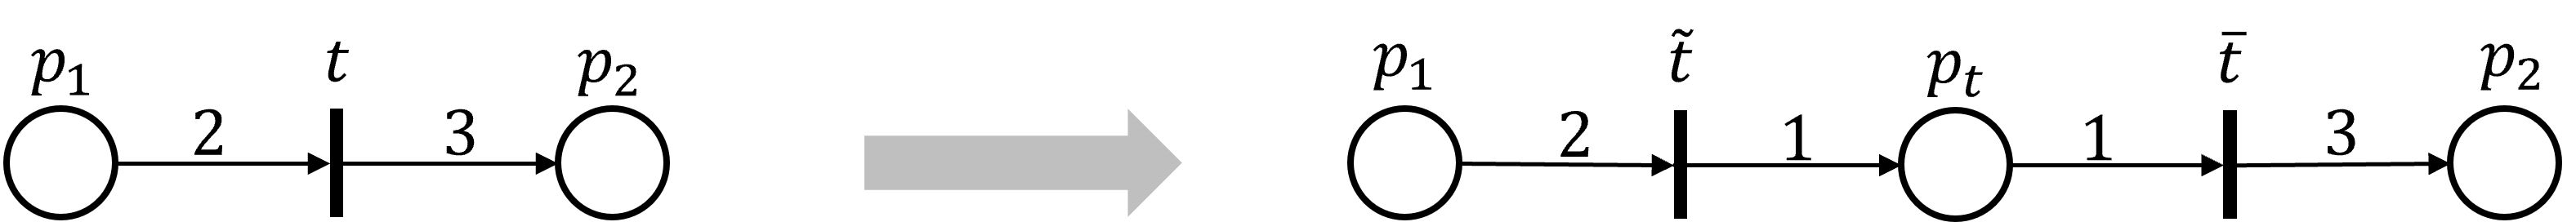
\includegraphics[width=0.8\textwidth]{Figures/TPN_expansion.png}
	\caption{TPN expansion.}
	\label{fig:tpn_expansion}
\end{figure}


\subsection{Event sequencing constraints}
The index $i$ of event $e^{t,s}_i$ represents the sequence of firing starting, i.e., if a firing starts in an earlier iteration, then its index will be smaller. Moreover, a firing must finish after starting. Group-C constraints force such sequences, which are relevant to all events. Constraints (C1) show that if the $i$-th firing of transition $t$ does not start before simulation termination, then the $(i+1)$-th firing will not start. Constraints (C2) state that if the $i$-th firing of transition $t$ does not start before simulation termination, then it will not finish. Constraints (C3) state that a firing cannot finish before starting, unless it remains in the future event list at the end of the simulation run. Constraints (C4) depict that the $(i+1)$-th firing of transition $t$ must be scheduled after the $i$-th execution, unless the $(i+1)$-th execution is not scheduled before simulation termination.
\begin{eqnarray}
	\sum_{k\in \mathbb{K}} x^{t}_{i+1,k} - \sum_{k\in \mathbb{K}} x^{t}_{i,k} \le 0&  \forall\ t\in \mathbb{T},i\in \mathbb{I}^{t}&(C1)\nonumber\\
	\sum_{k\in \mathbb{K}} w^{t}_{i,k}-\sum_{k\in \mathbb{K}} x^{t}_{i,k} \le 0&  \forall\ t\in \mathbb{T},i\in \mathbb{I}^{t}&(C2)\nonumber\\
	\sum_{k\in \mathbb{K}} kw^{t}_{i,k} - \sum_{k\in \mathbb{K}} kx^{t}_{i,k} \ge M(\sum_{k\in \mathbb{K}} w^{t}_{i,k}-1) &\forall\ t\in \mathbb{T}, i\in \mathbb{I}^{t}&(C3) \nonumber\\
	\sum_{k\in \mathbb{K}} kx^{t}_{i+1,k} - \sum_{k\in \mathbb{K}} kx^{t}_{i,k} \ge 1+M(\sum_{k\in \mathbb{K}} x^{t}_{i+1,k}-1)&  \forall\ t\in \mathbb{T},i\in \mathbb{I}^{t}&(C4)\nonumber
\end{eqnarray}

\subsection{State transitions}

The tokens in place $p$ are changed from $m^{p}_{k}$ to $m^{p}_{k+1}$ in iteration $k$, as in constraints (E1) and in lines 16 to 18 in Algorithm 1. The transitions $t$ that start in fire in iteration $k$ absorbs $A^{p,t}$ tokens from the precedent places $p$, and the firing that finish in iteration $k$ releases tokens to the successive places. 

\begin{eqnarray}
	m^p_{k+1} = m^p_k - \sum_{t\in \mathbb{T}} W^{p,t} \sum_{i\in \mathbb{I}^{t}} x^t_{i,k} +  \sum_{t\in \mathbb{T}} W^{t,p} \sum_{i\in \mathbb{I}^{t}} w^t_{i,k} &\forall p\in \mathbb{P}, k\in \mathbb{K}& (E1) \nonumber
\end{eqnarray}

\subsection{Objective function}\label{sec:TPN_obj}
With the constraints defined in the previous sections, there is a unique feasible solution in terms of transition firing times and the history of simulation clock, i.e., $e^{t,s}_i$, $e^{t,f}_{i}$ and $\mathcal{E}_k$. Thus, the objective function can be any function of those variables, for instance, average of system time or waiting time in queueing systems. Multiple feasible solutions may appear in terms of binary variables, since the sequence of events with identical execution time is not uniquely defined.

The flexibility of the objective function definition is a main difference between the formulation proposed by \cite{chan2008optimization} and this work, since the objective function of MPR in \cite{chan2008optimization} can be only the sum of all execution times. The uniqueness of optimal solution and flexibility of objective function formulation is particularly beneficial if one wants to make use of the resulting MPR to solve an optimization problem concerning the design or operation of the discrete event system (for instance the capacity of the queue or the control policy of a manufacturing system), since changing the objective function or adding new constraints to calculate the system performance will not influence the equivalence of MPR and a simulation run. %This issue will be discussed in Section 4.


\section{Applications}
In this section, several examples are presented, including a G/G/m queue, a merge queueing system composed by three single server stations, and a single server queue with failure as an example of event cancellation. The equivalence of MPR solution and history of a simulation run has been validated with $K$ equal to 20 for 100 independent replicates. 

\subsection{G/G/m queue}\label{sec:TPN_ggm}
The first example is a G/G/m queue, and the TPN is shown in Figure \ref{fig:tpn_GG2}. In a G/G/m queue, customers arrive at the queue following an general arrival process. One of the identical idle servers processes customers in the queue one by one, and the processing time is generally distributed. After processing, the customer will be released from the system immediately, and the server becomes idle again. In Figure \ref{fig:tpn_GG2}, the TPN of the TPN of G/G/2 is presented. A token in place $p_{arr}$ shows that it is possible to schedule the arrival of next customer, and the firing time of transition $t_{arr}$ is equal to the inter-arrival time. At the end of firing $t_{arr}$, a customer arrives, and it is possible to schedule the next arrival, thus, it releases one token to $p_{arr}$. Furthermore, an arrival will increase the length of the queue by 1, which is represented by the number of tokens in place $p_{queue}$. Two tokens in place $p_{idle}$ shows that two servers are idle. The firing of transition $t_{process}$ shows the processing of a customer, and it is enabled if and only if at least one server is idle and there is a customer in the queue. Once the process of the customer finishes, i.e., the end of firing $t_{process}$, a server is released, and a token is sent to place $p_{idle}$.

\begin{figure}[h]
	\centering
	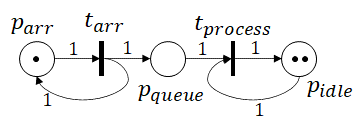
\includegraphics[width=0.45\textwidth]{Figures/TPN-GG2.png}
	\caption{TPN of G/G/2.}
	\label{fig:tpn_GG2}
\end{figure}

As mentioned in Section \ref{sec:MPR_start_Firing}, the transitions with non-zero firing times are expanded before implementing the MPR generation. The expanded TPN of the G/G/2 queue is shown in Figure \ref{fig:tpn_GG2_expansion}. Transition $t_{process}$ is expanded to $\tilde{t}_{process}$, $\bar{t}_{process}$ and $p_{process}$. Even though transition $t_{arr}$ also has non-zero firing time, it is self-limiting, i.e., there is never more than one firing in process. Therefore, it is not necessary to expand transition $t_{arr}$.

\begin{figure}[h]
	\centering
	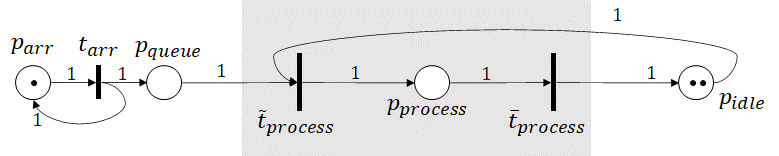
\includegraphics[width=0.8\textwidth]{Figures/TPN-GG2-expansion.png}
	\caption{TPN expansion of G/G/2.}
	\label{fig:tpn_GG2_expansion}
\end{figure}

The MPR of G/G/m queue is presented in the follows. The set of transitions $\mathbb{T}$ is specified by $\{t_arr, t_queue,\tilde{t}_{process}, \bar{t}_{process}\}$ for G/G/m queue. The constraints 


Table \ref{tab:sim_GGM} shows a simulation run of a G/G/m queue including 10 executions. In iteration zero, the system is in initial state, and this state satisfies the condition to schedule the counting event of arrival, as in lines 2 to 8 in Algorithm 3. In the solution of MPR, the scheduling of $\tilde{arr}$ is represented by $z^{\tilde{arr}}_0$ and $x^{\tilde{arr}}_{1,0}$ equal to 1, and its occurring time is equal to the simulation clock, which is equal to 0. The execution $(\tilde{arr}, 1, e^{\tilde{arr},0}_1, e^{\tilde{arr},1}_1)$, denoted by $e^{\tilde{arr}}_1$ in the table, is then performed since it is the earliest execution (line 18 in Algorithm 3), which is also indicated by $w^{\tilde{arr}}_{1,1}$ equal to one, and simulation clock in the next iteration, i.e., iteration $1$, is equal to the occurring time $e^{\tilde{arr}}_{1,1}$ in the solution of MPR. After that, the positive-delay event $arr$ is then scheduled (lines 26 to 30 in Algorithm 3), which can also be seen from the MPR solution, since $x^{arr}_{1,1}$ is equal to one, the scheduling time of $e^{arr}_{1,0}$ is equal to the current simulation clock time and the occurrence time is 2.3 time unit later than the scheduling time, where 2.3 is sampled from the distribution of inter-arrival time $T^{arr}$. At the end of the iteration, the system state is updated according to the state transition function of event $\tilde{arr}$ (line 25 in Algorithm 3), which in the MPR solution is indicated by an increment equal to one of state variable $u^{arr}$. This procedure is repeated in the next iterations, and the equivalence of DES procedure and the solution of MPR can be seen from Table \ref{tab:sol_GGM}. 

\begin{landscape}
\begin{table}
	\caption{Simulation run and MPR solution of G/G/m queue.}
	\label{tab:sim_GGM}
	\begin{tabular}{llllll}
		\hline
		$k$ & $clock$& Markings & Start firings & Unfinished firings & Finish Firing  \\ \hline
		
		0 &0 & $(1,0,0,2)$& $t_{arr}$ & $t_{arr}:2.3$ & $t_{arr}:2.3$ \\
		   &$\mathcal{E}_0=0$   &$\mathbf{m}_0 = (1,0,0,2)$ & $z^{arr}_{0} = 1, x^{arr}_{1,0}=1, e^{arr,s}_{1}=0, e^{arr,f}_{1}=2.3$ & & $w^{arr}_{1,0}=1$ \\ \hline
		
		1 & 2.3 & $(1,1,0,2)$ & $t^{arr},\tilde{t}_{proc}$ & $\tilde{t}_{proc}:2.3, t^{arr}:11.1$ & $\tilde{t}_{proc}:2.3$ \\
		& $\mathcal{E}_1=2.3$ & $\mathbf{m}_1 = (1,1,0,2)$ & $z^{arr}_{1} = 1, x^{arr}_{2,1}=1, e^{arr,s}_{2}=2.3,  e^{arr,f}_{2}=11.1$ & & $w^{\tilde{proc}}_{1,1}=1$ \\ 
		&  &  & $z^{\tilde{proc}}_{1} = 1, x^{\tilde{proc}}_{1,1}=1, e^{\tilde{proc},s}_{1}=2.3, e^{\tilde{proc},f}_{1}=2.3$ & &  \\ \hline
		
		2 & 2.3 & $(0,0,1,1)$ & $\bar{t}_{proc}$ & $\bar{t}_{proc}:6, t^{arr}:11.1$ & $\bar{t}_{proc}:6$ \\
		 & $\mathcal{E}_2=2.3$&$\mathbf{m}_2=(0,0,1,1)$&$z^{\bar{proc}}_{2} = 1, x^{\bar{proc}}_{1,2}=1, e^{\bar{proc},s}_{1}=2.3, e^{\bar{proc},f}_{1}=6$ & & $w^{\bar{proc}}_{1,2}=1$ \\ \hline
		 
		 3 & 6 & $(0,0,0,2)$ & &	 $t^{arr}:11.1$ & $t^{arr}:11.1$\\
		   & $\mathcal{E}_3=6$ & $\mathbf{m}_3=(0,0,0,2)$ & & &$w^{arr}_{2,3}=1$ \\ \hline
		   
		 4 & 11.1 & $(1,1,0,2)$ & $t^{arr}, \tilde{t}^{proc}$ &  $ \tilde{t}^{proc}:11.1, t^{arr}:12.1$ & $\tilde{t}_{proc}:11.1$ \\
		 & $\mathcal{E}_4=11.1$ & $\mathbf{m}_4=(1,1,0,2)$ & $z^{arr}_{4} = 1, x^{arr}_{3,4}=1, e^{arr,s}_{3}=11.1,e^{arr,f}_{3}=12.1$ & & $w^{\tilde{proc}}_{2,4}=1, $ \\ 
		 &  &  & $z^{\tilde{proc}}_{4} = 1, x^{\tilde{proc}}_{2,4}=1, e^{\tilde{proc},s}_{2}=11.1, e^{\tilde{proc},f}_{2}=11.1$ & &  \\ \hline
		 
		 5 & 11.1 & $(0,0,1,1)$ & $\bar{t}_{proc}$ & $t^{arr}:12.1, \bar{t}_{proc}:16.9$ & $t^{arr}:12.1$ \\
		 & $\mathcal{E}_5=11.1$&$\mathbf{m}_5=(0,0,1,1)$&$z^{\bar{proc}}_{5} = 1, x^{\bar{proc}}_{2,5}=1, e^{\bar{proc},s}_{2}=11.1, e^{\bar{proc},f}_{2}=16.9$ & & $w^{arr}_{3,5}=1$ \\ \hline
		 
		 6 & 12.1 & $(1,1,0,1)$ & $t^{arr}, \tilde{t}^{proc}$ & $\tilde{t}^{proc}:12.1, t^{arr}:15.2, \bar{t}_{proc}:16.9$ & $\tilde{t}^{proc}:12.1$\\
		& $\mathcal{E}_6=12.1$ & $\mathbf{m}_6=(1,1,0,1)$& $z^{arr}_6=1, x^{arr}_{4,6}=1, e^{arr,s}_{4}=12.1, e^{arr,f}_{4}=15.2$ && $w^{\tilde{proc}}_{3,6}=1$ \\
		&  & & $z^{\tilde{proc}}_6=1, x^{\tilde{proc}}_{3,6}=1, e^{\tilde{proc},s}_{3}=12.1, e^{\tilde{proc},f}_{3}=12.1$ &&  \\ \hline
		
		7 & 12.1 & $(0,0,1,0)$ &$\bar{t}^{proc}$ & $t^{arr}:15.2, \bar{t}^{proc}:16.9, \bar{t}^{proc}:20.1$ & $t^{arr}:15.2$ \\
		&  $\mathcal{E}_7=12.1$ &$\mathbf{m}_7=(0,0,1,0)$ & $z^{\bar{proc}}_{7} = 1, x^{\bar{proc}}_{3,7}=1, e^{\bar{proc},s}_{3}=12.1, e^{\bar{proc},f}_{3}=20.1$ &  & $w^{arr}_{4,7}=1$\\ \hline
		
		8 & 15.2 & $(1,1,0,0)$ &  $t^{arr}$ & $\bar{t}^{proc}:16.9, t^{arr}:17.8, \bar{t}^{proc}:20.1$ & $\bar{t}^{proc}:16.9$\\
		& $\mathcal{E}_8=15.2$ & $\mathbf{m}_8=(1,1,0,0)$& $z^{arr}_{8} = 1, x^{arr}_{5,8}=1, e^{arr,s}_{5}=15.2, e^{arr,f}_{5}=17.8 $ &&$w^{\bar{t}^{proc}}_{2,8}=1$\\ \hline
		
		9 & 16.9 & $(0,1,0,1)$ & $\tilde{t}^{proc}$ & $\tilde{t}^{proc}:16.9, t^{arr}:17.8, \bar{t}^{proc}:20.1$ & $\tilde{t}^{proc}:16.9$\\
		& $\mathcal{E}_9=16.9$ & $\mathbf{m}_9=(0,1,0,1)$ & $z^{\tilde{proc}}_{9} = 1, x^{\tilde{proc}}_{4,9}=1, e^{\tilde{proc},s}_{4}=16.9,  e^{\tilde{proc},f}_{4}=16.9$ &&$w^{\tilde{proc}}_{4,9}=1$\\ \hline
		
		10 & 16.9 & $(0,0,1,0)$ & $\bar{t}^{proc}$ & $t^{arr}:17.8, \bar{t}^{proc}:20.1, \bar{t}^{proc}:25.5$ & $t^{arr}:17.8$\\
		& $\mathcal{E}_{10}=16.9$ & $\mathbf{m}_{10}=(0,0,1,0)$ & $z^{\bar{proc}}_{10} = 1, x^{\bar{proc}}_{4,10}=1, e^{\bar{proc},s}_{4}=16.9,  e^{\bar{proc},f}_{4}=25.5$&&$w^{arr}_{5,10}=1$\\
		
		\hline
 	\end{tabular}
\end{table}
\end{landscape}




\section{Introduction}
Discrete Event Simulation (DES) is one of the most used tools for performance evaluation of %discrete event dynamic
complex systems in manufacturing and service applications. Hence, simulation--optimization algorithms are widely used %developed for optimizing the parameters of such systems. 
when performance evaluation must be coupled with optimization, i.e., when the best system configuration, according to some criteria, has to be found meanwhile guaranteeing a given value of some performance measure.  
Most of the state--of--the--art simulation--optimization algorithms consider DES as a \textit{black--box} function, and the structure of DES models has been seldom studied. On the contrary, a minority of the simulation--optimization literature explores the structure of the DES models, and %that
such approaches are referred to as \textit{white--box} simulation--optimization. 
Under the black--box setting, simulation--optimization algorithms work in an iterative way, alternating simulation and optimization procedures, 
thus, possibly leading to computational inefficiency if the number of iterations and/or the computation time per iteration increases too much. 
%and always require %huge amount of 
%many iterations to explore the %search 
%feasible region of the optimization problem, %and can be
%thus possibly leading to %computationally inefficient. 
%computational inefficiency.
The benefit of white--box simulation--optimization is the saving of simulation budget or computation time since 
the optimization procedure is guided by the information contained in the structure of the DES model (\cite{zhang2020sample}). However, the barrier to the use of white--box simulation--optimization is modeling DES as white box, so that it eventually favors optimization. 

%When there is already a DES model, 
The benefit of developing an MPR might be not obvious (especially when there is already a DES model) due to the extremely high complexity of solving it. 
%One may be confused about the motivation of this work, i.e., why one wants the MPR when he/she has already a simulation model at hand, since the complexity of solving mathematical programming is usually high. 
However, this work does not suggest solving the MPR directly with state-of-the-art optimizers. Instead, the optimal solution of the MPR can be obtained from a simulation run. The added value of the MPR is that the structure of the DES can be explored. With the vast theoretical and methodological results developed in the mathematical programming (MP) field, for instance sensitivity analysis as suggested by \cite{chan2008optimization}, the MPR of a simulation model favors the optimal design and control of the discrete event systems. 

This work proposes a procedure to establish a white--box simulation model, which is an equivalent Mathematical Programming Representation (MPR) model, based on the well-known event--scheduling logic (\cite{law2014simulation}). %for  
The procedure is applicable to certain types of DES models, and the assumptions that the DES model should satisfy are also presented in this work.
%Specifically, the modeling procedure, the assumptions which the DES model has to satisfy so that it can be applied and some examples are discussed. 

%In this work, we present how to establish an equivalent Mathematical Programming Representation (MPR) of Discrete Event Simulation (DES). The MPR depicts the dynamics of an event-scheduling approach of simulation modeling with a certain sample path. To develop the MPR, state variables, events, initial state, termination condition and the samples of the random variate should be provided. All requirement is also essential each time an event-scheduling algorithm is programmed. Furthermore, the proposed approach is quite routined. Thus, no extra knowledge or skills are required when one has the event-scheduling simulation implementation and wants to apply our approach. Besides the modeling approach, we provide the conditions to check before applying our approach, and discuss what the modifications can be done when some conditions are violated. Some examples are also given.

%Considering the literature on simulation--optimization, 
\cite{chan2008optimization} proposed a modeling framework to translate a DES model into an MPR model in a general sense. Their modeling framework is based on the Event Relationship Graph (ERG) of the system dynamics. To derive the MPR, % model, 
an ERG of the DES must be constructed and expanded to an elementary ERG (EERG) model, and a procedure can be applied to translate the EERG model into an MPR. %model. 
However, this procedure has some limitations. First, deriving an ERG is not an easy task, and the user must pay quite much attention to detect all the event relationships and complete the triggering conditions between each pair of related events. %That 
The difficulty of developing ERG limits the wide spread of this procedure. 
Second, the modeling procedure is case--by--case depending on the event relationships, which means that the user must analyze the event relationships one by one and identify which type of modeling, including the variables and constraints, he/she should apply for each event relationship. Consequently, an automatic procedure was not proposed. 
%which means the user has to first identify which situations he/she faces by analyzing the relationships between each couple of events in the EERG, and then choose the appropriate model, including the variables and constraints. 
This is quite %a burden
difficult, since EERG is an expansion of ERG; the resulting graph could be huge and writing down the complete MPR model could be even impossible.  

This work proposes a procedure that does not need % without plotting 
the ERG and %the modeling procedure 
can be used to automatically generate the MPR in a general--purpose programming language. Despite %taking different paths
being different, the MPRs proposed in this work and \cite{chan2008optimization} lead to %the 
equivalent results, which, in turn, are both equivalent to a simulation realization. The procedure can also be applied to devise MPR of DES with event cancellation, which was not considered in the work of Chan and Schruben (2008).


Many works in the literature show the potentiality of this research direction. For instance, the gradient can be conveniently estimated from the simulation model, if the MPR is approximated into Linear Programming (LP) and %solving 
the dual can be conveniently obtained (\cite{chan2008optimization}). Moreover, if some of the parameters in the MPR are changed to decision variables, the MPR becomes an integrated simulation--optimization model. Solving the integrated model provides the optimal solution of the optimization problem (\cite{matta2008simulation}). MP--based algorithms, such as linear programming approximation (\cite{alfieri2012mathematical}), Benders decomposition (\cite{weiss2015buffer}), row-column generation (\cite{alfieri2020time}), have been applied to improve the efficiency of %solving the 
integrated MP model solution. 


The application of MPR--based simulation--optimization approaches is usually found in operations management of manufacturing and service systems. %The integrated simulation--optimization model has proved itself to be well suited in solving the buffer allocation problem \citep{zhang2020BAP}. %The most efficient approach to finding the sample--path global optimal of the buffer allocation problem of serial production line is developed based on it \citep{zhang2020BAP}. 
%Thanks to the flexibility of DES in evaluating complex systems, the buffer allocation problem of production systems with complex blocking mechanism, such as kanban control, base stock control, extended kanban control, can be managed \citep{pedrielli2015integrated}. Thanks to the flexibility of MPR in modeling optimization problems, problems involving real--valued decision variables such as optimal production rate \citep{tan2015mathematical}, bottleneck detection and throughput improvement problem \citep{zhang2020models} have all been well addressed and the sample--path global optimal solution can be obtained. %It is worthy to notice that, 
The flexibility of DES for complex system evaluation and of MPR for modeling optimization problems, allowed the integrated simulation-optimization approach to be effectively applied to buffer allocation problems (\cite{zhang2020BAP}), even with complex blocking mechanisms (\cite{pedrielli2015integrated}) and to problems involving real value decision variables (\cite{tan2015mathematical,zhang2020models}). 
Before the above-mentioned works were proposed, there were many state--of--the--art heuristic approaches addressing those problems, but without any guarantee of global or local optimality. Thus, the development of MPR--based simulation--optimization has made its contribution in the research area of manufacturing and service system optimization.

%To extend the application of the MPR-based simulation optimization approaches, there is a need of modeling approach to translating DES into MPR under general settings.

The contributions of this work are several and refer to different aspects. First, it proposes an MPR of DES from event-scheduling execution logic, which is the foundation of many DES implementations. Thus, the procedure does not require much extra effort once one has an event-scheduling execution logic implemented, while the state-of-the-art approach requires the DES modeled with ERG. The proposed approach can be easily automated (the source code has been uploaded in a repository, as explained in the following).  Second, it proposes the MPR of event cancellation, which is usually used to model queue with abandonment or servers with failures but has never been studied in the literature. This work will be a foundation of developing math-programming-based simulation-optimization algorithm, based on the vast literature in mathematical programming filed, for instance, the gradient estimation. 
%Third, the vast literature in mathematical programming field can be applied to the resulting MPR, for instance, for gradient estimation. Last, 
The proposed MPR can also be easily transformed into an MPR for optimizing the design parameters of the DES, which are common optimization problems in operations management field.  


The rest of the paper is organized as follows. Section \ref{sec:MPR} describes the generation of the MPR of a DES model, including a brief introduction of event-scheduling algorithm, the assumptions for applying the proposed procedure, a modified event-scheduling algorithm, and the MPR itself automatically generated based on the model. Section \ref{sec:app} shows several examples of DES and the generated MPR, whose equivalence has been validated. Result discussion and conclusion are reported in Section \ref{sec:discussion} and \ref{sec:conclusion}, respectively.


\section{MPR generation procedure} \label{sec:MPR}
\subsection{Event-scheduling execution logic of DES } \label{sec:SimAlgo}
The event-scheduling approach is the logic behind all the major DES software and used by practitioners when developing simulation codes with general purpose languages (\cite{law2014simulation}). For sake of completeness, the logic is briefly described. The fundamental elements are the \textit{system state} and the \textit{events}. The system state $\textbf{s}$ is a set of state variables $s$ needed to describe the system at a particular time. An event $\xi$ is composed by a collection of four objects, $(CS^{\xi}(\textbf{s}),\ CC^{\xi}(\textbf{s}),\ F^{\xi}(\textbf{s}),\ T^{\xi})$, where:
\begin{eqnarray}
	CS^{\xi}(\textbf{s}): && \text{condition to schedule}\nonumber\\
	CC^{\xi}(\textbf{s}): && \text{condition to cancel}\nonumber\\
	F^{\xi}(\textbf{s}): && \text{state transition function}\nonumber\\
	T^{\xi}: && \text{delay between schedule and occurrence.}\nonumber
\end{eqnarray}
Condition to schedule and to cancel an event are logic expressions based on the system state $\textbf{s}$, and the output will be true if the system state allows to schedule or cancel executions. The occurrence of an event changes the system state, which is indicated by the state transition function. The input and output of $F^{\xi}(\textbf{s})$ are the system state before and after event occurrence, respectively. There is a delay, zero or positive, between scheduling time and occurring time, and this delay is called \textit{occurrence delay} and denoted as $T^{\xi}$ in the rest of the paper. In this work, $T^{\xi}$ is considered as random variate. Generally, each event usually occurs more than once during a simulation run, and the term \textit{execution} is introduced to specify a certain occurrence of an event. An execution is composed by a set of four objects, $(\xi,i,\tau_0,\tau_1)$, where $\xi$ denotes the event type, $i$ denotes the index of execution, $\tau_0$ denotes the scheduling time and $\tau_1$ denotes the occurring time. 

Given a set of events $\mathbb{X}$, initial system state $\textbf{s}_0$, and simulation length defined as the number of iterations and denoted by $K$, a DES model could be implemented with the event-scheduling logic, as in Algorithm 2. The algorithm is initialized with simulation the clock equal to zero, number of executions scheduled in the past for each event type equal to zero, and empty future event list. The \textit{future event list} is a list of executions, which are scheduled but not occur yet. Each iteration is composed by three steps, which are scheduling new executions, canceling executions and performing an execution. First, for each event type $\xi$, if the condition to schedule $\xi$ is true, a new execution of $\xi$ is created and added to the future event list, as in lines 3 to 9. Then, for each execution in the future event list, if the condition to cancel the event is true, the executions of that event type is removed from the future event list, as in lines 12 to 16. Finally, the execution with the earliest occurring time is taken from the future event list, the system state is changed according to the state transition function of the event type, and the simulation clock is set to the occurring time. If there are more than one execution with the same earliest occurring time, the algorithm can randomly pick one among them or according to a priority rule.
%The event-scheduling approach is the logic behind all the major DES software and used by practitioners when developing simulation codes with general purpose languages \citep{law2014simulation}. For sake of completeness, the logic is briefly described as shown in Figure \ref{Fig:SimAlgo}. The fundamental elements are the system state and the events. The system state is a collection of state variables to describe the system at a particular time, while an event is everything whose execution can change the system state. All the already scheduled but not yet executed events are stored in the future event list together with their occurring times. When simulation is launched, the system state and the future event list is initialized with user-defined values, and the simulation clock is set to zero. The event with the earliest occurring time in the future event list will be executed, and the system evolves into a new state together with the simulation clock. The new state may enable to schedule new events, i.e., adding new event together with execution time to the future event list, or cancel events, i.e., removing some event executions from the future event list. There is usually a delay between the time when an event is added to the event list and the time when the event is executed. In the following, we refer the time when an event is added to the event list as the \textit{scheduling time}, and the time when an event is executed as the \textit{execution time}. The algorithm will terminate when some given condition is met or when a given value for the simulation clock is reached.

%\begin{figure}[h]
%	\centering
%	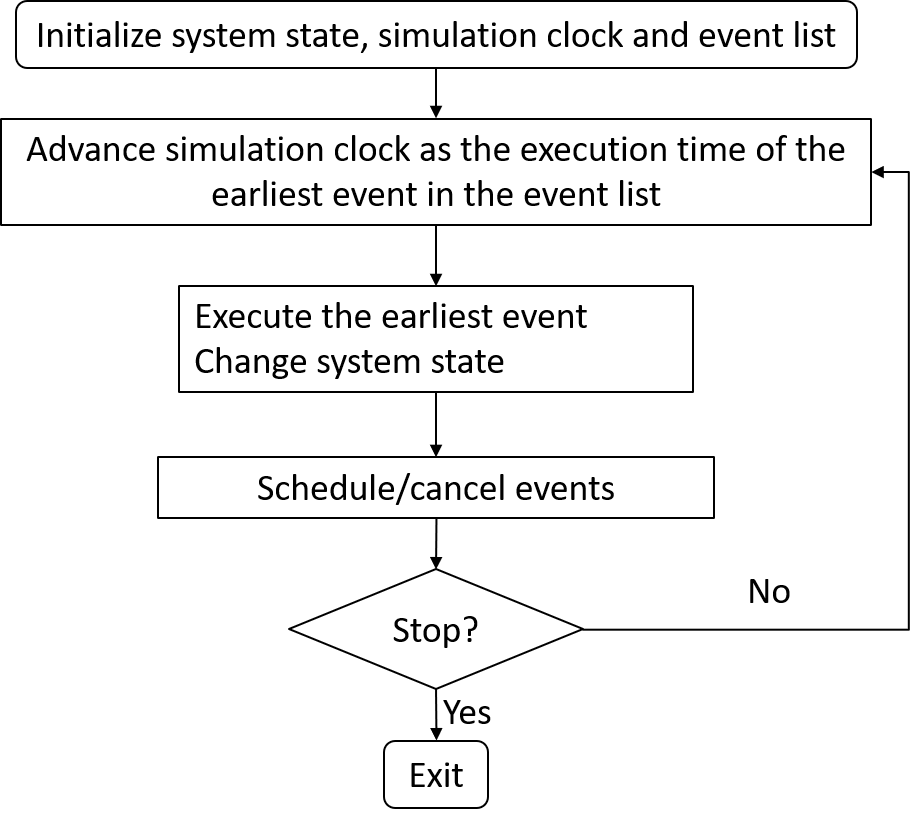
\includegraphics[width=0.6\textwidth]{Figures/EventSimAlgo.png}
%	\caption{Event-scheduling simulation algorithm.}
%	\label{Fig:SimAlgo}
%\end{figure}

%\section{Mathematical programming representation of DES}
In the following, a procedure to translate DES models into MPR models, based on the event-scheduling logic, is introduced. Before presenting the procedure, the assumptions that the DES model has to satisfy in order to have the procedure applicable, are introduced.

\subsection{Assumptions}
To apply the procedure proposed in this work, the following assumptions must be satisfied.

\begin{enumerate}
	\item State variables are integer.
	\item For all the event types $\xi$, the \textit{condition to schedule} and the \textit{condition to cancel} are in the form $a^{\xi,s}\le s \le c^{\xi,s}$, where $a^{\xi,s}$ and $c^{\xi,s}$ are integers and represent, respectively, the lower bound and the upper bound of a range, for a certain state variable $s$. When multiple state variables are involved, they are combined using the logical operator ``AND".
	%and combined with logic operator ``AND" when multiple state variables are involved, where $a^{\xi,s}$ and $b^{\xi,s}$ are given.
	%\item The scheduling condition of an event is independent of the history and not changed along time.% (It could be possible to define more state variables in case of history dependence and time-variant scheduling conditions.)
	%\item An event execution of $e^{\xi}$ leads to (integer) increment or decrement equal to $\Delta^{\xi}_s$ of certain state variables $s$, and $\Delta^{\xi}_s$ is not changed along time. (A direct evaluation can be modeled in this way.)
	\item The occurring delay of each execution can be generated off-line. %(\textit{This point is different from ERG. In ERG, the delay is dependent on the edge, i.e, a couple of events, but I consider delay dependent on a single event.})
	\item When more than one execution in the future event list have the same occurring time% as the earliest execution time
	, the sequence of performing the executions is immaterial, i.e., different sequences lead to the same new system state and the same new event list when the simulation clock is advanced.
	\item Only events with strictly positive occurrence delay can be canceled.
	%	the system state, the event list and the number of past executions of each event type are independent of the sequence of execution when the simulation clock is advanced.
	%\item Simulation terminates when the total number of executions reaches a known value $K$.
	%Simulation terminates when the number of execution of each event $e^{\xi}$ reaches $N^{\xi}$, which is known, i.e., the number of entities in the system is known. 
	%\item Only event with positive-delay between scheduling and execution can be canceled.
\end{enumerate}

The first assumption requires the state variables to be integer. Integer variables widely exist in DES models, such as number of jobs in buffers, idle servers, and binary variables to model system behavior and control. A discrete state variable can be translated into an integer variable or a set of binary variables. For real-valued state variables, they can be approximately discretized. Thus, the first assumption is fairly general.

The second assumption is, instead, more strict. However, if a model does not satisfy this condition, one can consider to introduce extra binary variables to satisfy assumption (2). For instance, if the condition to schedule executions of event type ${\xi}$ is $s\le a^{\xi,s} \ OR\ s\ge c^{\xi,s}$, a binary variable $s^{'}$ can be introduced in the model, and $s^{'}$ is equal to one if and only if 
$s\le a^{\xi,s} \ OR\ s\ge c^{\xi,s}$. Thus, violation of assumption (2) can be overcome, even though at the cost of an increase of the model complexity.

As for the third assumption, the delay represents usually inter-arrival time or service time in queueing systems. These delays will be used as the constant term of some constraints in the proposed MPR, hence, they should be generated offline, i.e., independently from the real-time state of the system. For instance, both stationary and non-stationary arrival process will satisfy this assumption.
%For example, if an event represents the finishing of a job on a machine, it is scheduled (i.e., put in the list) when the job starts its processing, and it will be executed when the jobs will be finished, i.e., the time between scheduling and execution is the job processing time. 
%If the condition is not met, i.e., if the occurrence delay is not iid, it can be splitted into several events so that each event has iid delay. For instance, if the distribution of service time depends on the job type, the event of \textit{finishing} a job should be splitted such that the \textit{finishing} of each job type is represented by one event. 

The fourth assumption, in practice, says that the execution time is the only attribute of priority for the event executions in the future event list. If one would like to specify a different priority for events having the same execution time, he/she can specify the priority by adding the event with lower priority to the event list after the execution of the event with higher priority, which can be done by introducing extra binary variables. 


The fifth assumption is an extension of the fourth one. Assumption (4) implies that only events with positive delay can be canceled. Let us assume that there is a zero-delay event ${\xi}$ with cancellation. After an execution, $(\xi,i,\tau_0,\tau_0,false)$, is added to the future event list in iteration $k$. It is obvious that the condition to schedule and the condition to cancel an event are not identical; thus, either the new execution must occur immediately if there is no other execution in the future event list having the same occurring time $\tau_0$ and event cancellation is not relevant, or there are such executions and two cases can occur. In one case, execution $(\xi,i,\tau_0,\tau_0,false)$ is immediately executed in iteration $(k+1)$. In the other case, if some other executions with occurring time equal to $\tau_0$ are executed earlier than execution $(\xi,i,\tau_0,\tau_0,false)$, and the condition to cancel $\xi$ is true at a certain time, then the execution $(\xi,i,\tau_0,\tau_0,false)$ is canceled and never occurs. The simulation realization in the latter case is different from the former one, and assumption (4) is violated. Thus, only positive-delay event can be canceled.
%The fifth condition specifies termination condition of the event-scheduling algorithm. %Specifically, for queueing systems, the termination condition usually refers to the number of jobs passing through each station.


%The proposed procedure cannot handling event cancellation, as stated in the last assumption.

\subsection{Modified event-scheduling execution logic} \label{sec:MPR_procedure}

It is not trivial to generate an MPR based on Algorithm 2. Thus, a modified event-scheduling execution logic is proposed this modified algorithm is equivalent to Algorithm 2, but enables the MPR generation. In the modified algorithm, each event is categorized as zero-delay or positive-delay, depending on whether the occurrence delay $T^{\xi}$ is equal to zero with probability equal to one or not. The modifications differ for zero-delay and positive-delay events. 

In Algorithm 2, there may be more than one execution of the event type $\xi$ in the future event list. The first modification is that the number of executions of any zero-delay event in the future event list at any time is no more than one. Multiple executions are equivalent to sequentially schedule a new execution after the previous one occurs. 

The second modification is about the scheduling of positive-delay events. A \textit{counting event} ${\tilde{\xi}}$ and a counting variable $u^{\xi}$ are artificially created. The counting event ${\tilde{\xi}}$ is zero-delay, with the same scheduling condition as ${\xi}$. The simulation logic is then modified as follows. When the system state satisfies the condition to schedule $\xi$, an execution of event $\tilde{\xi}$, other than $\xi$, is added to the future event list. Only after event ${\tilde{\xi}}$ occurs, an execution of event type ${\xi}$ is added to the future event list. The counting variable $u^{\xi}$ represents the number of executions of ${\xi}$ in the future event list, and its value is incremented by one when counting event ${\tilde{\xi}}$ occurs and decremented by one when event ${\xi}$ occurs. 

The third modification is about event cancellation. A fifth object named \textit{cancel} is introduced to an \textit{execution}, which has a binary value indicating if the execution is canceled. It is initialized as \textit{false} (i.e., zero) when an execution is created. Once the condition to cancel executions of event type $\xi$ is true, the value of \textit{cancel} of those executions is changed to \textit{true}, (i.e., one), the counting variable $u^{\xi}$ is set to zero, but the execution is not removed from the future event list. When a canceled execution is taken from the future event list, the system state will remain unchanged and the algorithm will continue to the next iteration. 

Based on the assumptions and the three modifications above, compositions of zero-delay and positive-delay events can be modified accordingly. Zero-delay events are composed by a collection of two objects ($CS^{\xi}(\mathbf{s})$, $F^{\xi}(\mathbf{s})$), which are condition to schedule and state transition. Positive-delay events are composed by five objects ($T^{\xi}$, $\tilde{\xi}$, $u^{\xi}$, $CC^{\xi}(\mathbf{s})$, $F^{\xi}(\mathbf{s})$), which are occurrence delay, counting event, counting variable, condition to cancel and state transition, respectively.

The last modification is that besides integer $K$, which represents the total number of iterations, the number of executions of each event $\xi$, denoted by $N^{\xi}$, should also be provided. It is not necessary that $N^{\xi}$ is exactly equal to the number of executions of event $\xi$ in the simulation run, instead, it could be an upper bound. Generally speaking, $N^{\xi}$ can be equal to K, but the smaller the value, the smaller the number of variables, thus, a simpler model will be consequently developed. Since $N^{\xi}$ is not the exact number of executions of event $\xi$, when the simulation terminates, the future event list sometimes can be not empty, i.e., some executions are scheduled but never occur.

The modified event-scheduling logic is shown in Algorithm 3. The differences between the two algorithms are the following. In each iteration, only zero-delay events are scheduled by validating the condition to schedule, as in line 3. Positive-delay events are scheduled after the execution of its counting event is performed, as in lines 26 to 30. Canceled executions are not removed from the future event list, but the attribute \textit{cancel} is set to true, and the counting variable is set zero, as in line 13. When performing an execution, only the transition function of uncanceled executions will be applied, as in lines 21 to 23. 

%The condition to schedule, the condition to cancel, the distribution of delay between scheduling and execution $T^{\xi}$ should satisfy the assumptions (2) and (3). In the future event list, there is usually an upper bound on number of executions of the each event $e^{\xi}$, represented by $\beta^{\xi}$. For instance, to simulate an arrival process, the maximum number of arrivals in the event list is equal to $1$, since a new arrival can only be scheduled by the previous one, with a delay equal to the inter-arrival time. In the future event list, there may be one or more executions of the same event $e^{\xi}$. Events with $\beta^{\xi}$ equal to one, are named \textit{single-execution} events, and events with $\beta^{\xi}$ greater than one are named \textit{multi-execution} events. All the zero-delay events are defined as single-execution because, when the delay between scheduling and execution of an event is zero, multiple executions are equivalent to the sequential scheduling of a single-execution event. For positive-delay events $e^{\xi}$, the following procedure is introduced. A \textit{counting} event ${e}^{\tilde{\xi}}$ and counting variable $u^{\xi}$ are created artificially. The counting event ${e}^{\tilde{\xi}}$ is zero-delay, with the same scheduling condition as $e^{\xi}$. Each time the condition to schedule is true, an execution of ${e}^{\tilde{\xi}}$ is added to the future event list. When ${e}^{\tilde{\xi}}$ is actually executed, an execution of $e^{\xi}$ is added to the future event list. Then, if the condition to schedule event $e^{\xi}$ is still true, another ${e}^{\tilde{\xi}}$ is scheduled, therefore, simultaneous scheduling of multiple executions of event $e^{\xi}$ can be done in a sequential way without advancing simulation clock. The counting variable $u^{\xi}$ represents the number of executions of $e^{\xi}$ in the future event list, and its value is incremented by one when counting event $e^{\tilde{\xi}}$ is executed and decremented by one when event $e^{\xi}$ is executed. If event $e^{\xi}$ is canceled, $u^{\xi}$ is reset to zero. Since the maximum number of executions of $e^{\xi}$ is equal to $\beta^{\xi}$, the inequality $u^{\xi}\le\beta^{\xi}-1$ should be included into condition to schedule it, as well as event $e^{\tilde{\xi}}$. Besides integer $K$, which represents the total number of executions before simulation termination, the number of executions of each event $\xi$ should also be provided, denoted by $N^{\xi}$. It is not necessary that $N^{\xi}$ is exactly equal to the number of executions of event $\xi$ in the simulation run, instead, it could be an upper bound of it. Generally speaking, $N^{\xi}$ can be equal to K, but the smaller the value, the smaleler the number of variables that are, thus a simpler model will be developed consequently.


To summarize, to implement the modified event-scheduling logic, zero-delay events, including counting events of positive-delay events, must be provided together with the condition to schedule and the transition function, and positive-delay events must be provided together with occurrence delay, counting event, counting variable, condition to cancel and state transition function. An example of G/G/m queue is shown in Table \ref{tab:ggm_1}. Three events and two state variables are essential. The three events represent job arrival, service start and service finish, and are denoted by ${arr}$, ${ss}$ and ${sf}$, respectively. The two state variables represent the number of jobs in the queue and the number of occupied servers, and are denoted by $q$ and $g$, respectively. State variable $q$ is non-negative integer, and $g$ can be any integer between $0$ and $m$, which is the number of servers. Since event cancellation is not relevant to G/G/m queue, the condition to cancel is not showed. Event ${arr}$ is a positive-delay event, as explained above. %and one execution can be scheduled as soon as the previous job arrives with a delay equal to a sample from inter-arrival time distribution $T^{arr}$. 
A counting event of ${arr}$, i.e., ${\tilde{arr}}$, and a counting variable $u^{arr}$ are defined. The condition to schedule ${arr}$ is that $u^{arr}$ is equal to zero, since it is a renewal process, i.e., each time a job arrives, one and only one new arrival can be scheduled. When ${arr}$ is executed, one job arrives to the system, and queue level $q$ is increased by one. Event ${ss}$ is a zero-delay event. The condition to schedule ${ss}$ is that there is one job waiting in the queue and one server available. Upon execution of ${ss}$, queue level is reduced by one, and the number of occupied servers is increased by one. Event ${fs}$ is a positive-delay event, it is scheduled immediately after ${ss}$ is executed, and the delay until its execution is equal to the service time, i.e., sampled from $T^{sf}$. Therefore, event ${ss}$ can be regarded as the counting event of ${sf}$. Furthermore, state variable $g$ is the counting variable of ${sf}$. %If the simulation terminates with $N$ jobs processed by the system, the total number of executions of all events is equal to $N$.
The only information missing in the Table to complete the algorithm is number of iterations $K$ and number of executions of each event type $N^{\xi}$. 

%To derive the MPR of a simulation run of any system, one just needs state variables, zero-delay events and positive delay events as in Table \ref{tab:ggm_1}, number of iterations $K$ and number of executions $N^{\xi}$. Then, the MPR is derived as in next sections.

%To implement the event-schedule algorithm and generate MPR, events and state variables should be first defined. 
%For instance, to simulate a G/G/m system, three events and two state variables are essential. The three events represent job arrival, service start and service finish, and are denoted by ${arr}$, ${ss}$ and ${sf}$, respectively. The two state variables represent the number of jobs in the queue and the number of occupied servers, and are denoted by $q$ and $g$, respectively. State variable $q$ is non-negative integer, and $g$ can be any integer between $0$ and $m$, which is the number of servers. 

%To implement the event-scheduling logic in Algorithm 1, for each event $\xi$, the condition to schedule $CS^{\xi}$, the condition to cancel $CC^{\xi}$, the distribution of occurrence delay $T^{\xi}$ %, the maximum number of executions in the future event list $\beta^{\xi}$ and the state variable changes upon execution are also necessary. 
%and the state transition function must be provided. Besides, to derive the MPR with the proposed approach, some modifications must be made to the general event-scheduling algorithm in Algorithm 1, but the resulting algorithm will be equivalent. Each event is categorized as zero-delay or positive-delay, depending on whether the occurrence delay $T^{\xi}$ is equal to zero with probability equal to one or not. The modifications differ for zero-delay and positive-delay events. 

%\renewcommand\arraystretch{1.2}
\begin{table}[h]
	\begin{tabular}{llllll}
		\multicolumn{6}{l}{\textbf{State variables}}\\ \hline
		&&&&& Initial\\
		$s$ & \multicolumn{4}{l}{Description}& value\\\hline
		$g$& \multicolumn{4}{l}{Number of occupied servers}  & 0 \\
		$q$ & \multicolumn{4}{l}{Number of jobs in the queue} &0\\
		$u^{arr}$& \multicolumn{4}{l}{Number of executions with event type $arr$ }  &0\\
		&\multicolumn{4}{l}{in the future event list}& \\
		&&&&&\\
		\multicolumn{6}{l}{\textbf{Zero-delay events}}\\ \hline
		&&&&& State\\
		$\xi$&Description &  \multicolumn{3}{l}{Condition to schedule}& transition\\\hline%&$N^{\xi}$
		${\tilde{arr}}$ & Counting arrival&  \multicolumn{3}{l}{$u^{arr}\le0$} & $u^{arr}${\footnotesize++} \\
		${ss}$& Start 	& \multicolumn{3}{l}{$1\le q, g\le m-1$} & $g${\footnotesize++},$q${\small-}{\small-}  \\
		&&&&&\\
		\multicolumn{6}{l}{\textbf{Positive-delay events}}\\ \hline
		&&& Counting& Counting  & State \\
		$\xi$&Description & Delay &  event& variable & transition\\\hline
		${arr}$& Arrival & $T^{arr}$& ${\tilde{arr}}$& $u^{arr}$ & $q${\footnotesize++},$u^{arr}${\small-}{\small-} \\	
		${sf}$& Finish & $T^{sf}$& ${ss}$& $g$  & $g${\small-}{\small-} \\\hline
	\end{tabular}
	\caption{Events to simulate G/G/m system.}
	\label{tab:ggm_1}
\end{table}



\subsection{Mathematical programming model}

The MPR represents the dynamics of the simulated system, equivalent to the event-scheduling algorithm, i.e., Algorithm 3. Specifically, execution scheduling times, execution occurring times and state variable changes during the simulation run can all be seen in the MPR as decision variables. The scheduling times and the occurring times of the execution of event type $\xi$ indexed by $i$ are denoted by $e^{\xi,0}_{i}$ and $e^{\xi,1}_{i}$, respectively. Variables $\mathcal{E}_k$ denotes the simulation clock at the beginning of iteration $k$ in Algorithm 3. 
%The system state changes with event executions, and the executions are organized into a single series and $\mathcal{E}_k$ is used to denote the $k$-th execution time, i.e., the simulation clock values when an event occurs. In the rest of the paper, $i$ represents the index of the executions of a specific event, and index $k$ represents the index of execution of any event. 
Variables $e^{\xi,0}_{i}$, $e^{\xi,1}_{i}$ and $\mathcal{E}_k$ are all real-valued and non-negative. Variable $u^s_k$ is used to denote the value of state variable $s$ at the beginning of iteration $k$ in Algorithm 3%, i.e., just after the $k$-th execution, i.e., just after $\mathcal{E}_k$ and before scheduling or canceling any event
. Variables $u^s_k$ are integer according to assumption (1). Some binary variables are also used in the MPR, and they will be introduced in the following, during the explanation of the model. 

The set of all events $\xi$ is denoted by $\mathbb{X}$. $\mathbb{I}^{\xi}$ denotes the set $\{1,...,N^{\xi}\}$, which is the number of executions of event ${\xi}$, and $\mathbb{K}$ denotes the set $\{0,...,K\}$, which is the total number of executions in the simulation run. $\mathbb{S}$ denotes the set of all state variables. $\mathbb{S}^{\xi}$ and $\mathbb{S}^{\bar{\xi}}$ denote the set of state variables relevant to scheduling and cancellation conditions of event type ${\xi}$, respectively. $\mathbb{S}^{c}$ denotes the set of counting variables.

\subsubsection{Event execution} \label{sec:const_A}
The first group of mathematical relationships, denoted by group-A, are the constraints for performing one execution in one iteration of Algorithm 3. Binary variables $w^{\xi}_{i,k}$ are introduced to represent the $i$-th execution of event type $\xi$ occurring in iteration $k-1$. The $i$-th execution of event $\xi$ is performed in iteration $k-1$ if and only if $w^{\xi}_{i,k}$ is equal to one, and variable $e^{\xi}_{i,1}$ is binded to $\mathcal{E}_k$, as shown in constraints (A1) and (A2). Constraints (A3) state that in each iteration, one and only one execution occurs. Constraints (A4) state that an execution occurs at most once. 
%$e^{\xi,1}_i$ can be binded to at most one $\mathcal{E}_k$, while each $\mathcal{E}_k$ must be binded to one and only one $e^{\xi,1}_i$. 
Constraints (A5) imply that the simulation cannot be reversed from iteration $k-1$ to iteration $k$. 
%the subscript $k$ of $\mathcal{E}_{k}$ shows the sequence of execution, i.e., the simulation clock cannot be reversed from iteration $k-1$ to iteration $k$. 
Constraint (A6) implies that the simulation clock is initialized to zero. Constraints (A7) implies that the delay between the scheduling and occurrence of an execution is equal to a sample from the random variate $T^{\xi}$.
\begin{eqnarray}
	e^{\xi,1}_i-\mathcal{E}_k\ge M(w^{\xi}_{i,k}-1) & \forall\ \xi\in\mathbb{X},i\in \mathbb{I}^{\xi},k\in \mathbb{K}&(A1)\nonumber\\
	\mathcal{E}_k-e^{\xi,1}_i\ge M(w^{\xi}_{i,k}-1) & \forall\ \xi\in\mathbb{X},i\in \mathbb{I}^{\xi},k\in \mathbb{K}&(A2)\nonumber\\
	\sum_{k\in \mathbb{K}} w^{\xi}_{i,k} \le 1& \forall\ \xi\in\mathbb{X},i\in \mathbb{I}^{\xi}&(A3)\nonumber\\
	\sum_{\xi\in \mathbb{X}}\sum_{i\in \mathbb{I}^{\xi}} w^{\xi}_{i,k} =1&\forall\ k\in \mathbb{K}&(A4)\nonumber\\
	\mathcal{E}_{k}-\mathcal{E}_{k-1}\ge 0&\forall\ k\in \mathbb{K}&(A5)\nonumber\\
	%\sum_{k\in \mathbb{K}} kw^{\xi}_{i,k} - \sum_{k\in \mathbb{K}} kw^{\xi}_{i-1,k} \ge 1&  \forall\ \xi\in\mathbb{X},i\in \mathbb{I}^{\xi}&(A6)\nonumber\\
	\mathcal{E}_0 = 0&&(A6)\nonumber\\
	e^{\xi,1}_{i} - e^{\xi,0}_{i} = t^{\xi}_{i} & \forall \xi\in\mathbb{X}, i\in \mathbb{I}^{\xi}&(A7) \nonumber
\end{eqnarray}

%\subsubsection{Multiple-execution events}\label{sec:const_B}
%The second group of constraints, denoted by group B, are the constraints binding event scheduling $e^{\xi,0}_i$ and event execution $e^{\xi,1}_{i^{'}}$, and the time delay between which is a sample of $T^{\xi}$. If the event is single--execution, i.e., the maximum number of executions in the event list is equal to one, the $i$-th execution $e^{\xi,1}_i$ is the $i$-th scheduled one, as in constraints (B1), where $t^{\xi}_{i}$ is a sample of $T^{\xi}$. Thus, the variable $e^{\xi,1}_{i} $ can be replaced by $e^{\xi,0}_{i} + t^{\xi}_{i}$ and the MPR model can reduced.
%\begin{eqnarray}
%e^{\xi,1}_{i} - e^{\xi,0}_{i} = t^{\xi}_{i} & \forall \xi\in\mathbb{X}, i\in \mathbb{I}^{\xi}&(B1) \nonumber
%\end{eqnarray}

%If event $e^{\xi}$ is a multi-execution event, a late scheduled execution can overtake an early scheduled one, since the delay time between scheduling and execution is a random variate. For instance, in a G/G/2 queue, the departure of the first job is the first scheduled departure event, but it may be not the first to execute, if its service time is pretty long so that the second starting job leaves the system earlier. Thus, binary variables $y^{\xi}_{i,i^{'}}$ are introduced, and the $i^{'}$-th execution of event $e^{\xi}$ is the $i$-th scheduled one with a delay equal to $ t^{\xi}_{i}$, a sample of $T^{\xi}$, when $y^{\xi}_{i,i^{'}}$ is equal to one, as in constraints (B2) and (B3). Constraints (B4) and (B5) show that each execution can be binded to one and only one scheduling. Constraints (B6) imply that the $i$-th scheduling cannot be binded to an execution earlier than the $(i+\beta^{\xi})$-th, since at most $\beta^{\xi}$ executions are allowed to be in the list at the same time. For the same reason, constraints (B7) state that $i^{'}$-th execution cannot be binded to the scheduling later than the $(i^{'}-\beta^{\xi})$-th. For instance, in a G/G/2 queue, the third arrival job cannot be the first departure job, since its service starts after the first departure.

\subsubsection{Constraints for scheduling new events}\label{sec:const_B}
The second group of constraints, denoted by group B, state the scheduling of new executions. Binary variables $x^{\xi}_{i,k}$ are used to represent that an execution with event type $\xi$ and index $i$ is scheduled in iteration $k$ if it is equal to one. %., and $x^{\xi}_{i,k}$ equal to one represents that the $i$-th execution of event ${\xi}$ is scheduled in iteration $k$ in Algorithm 2, as in constraints (B1) and (B2). 
%that an execution of event $e^{\xi}$ can be scheduled right after $\mathcal{E}_k$ if the condition for scheduling an event $e^{\xi}$ is true. 
Constraints (B1) and (B2) shows that the scheduling time of the execution is equal to the simulation clock when it is scheduled.
\begin{eqnarray}
	e^{\xi,0}_i-\mathcal{E}_{k} \ge M(x^{\xi}_{i,k}-1)& \forall\ \xi\in \mathbb{X},k\in \mathbb{K},i\in \mathbb{I}^{\xi}&(B1)\nonumber\\
	\mathcal{E}_{k} -e^{\xi,0}_i\ge M(x^{\xi}_{i,k}-1)&\forall\ \xi\in \mathbb{X},k\in \mathbb{K},i\in \mathbb{I}^{\xi}&(B2)\nonumber
\end{eqnarray}

To schedule zero-delay events, the condition to schedule must be verified, as stated in lines 2 to 8 in Algorithm 3, and it is also shown by constraints (B3) to (B11). Binary variables $z^{\xi}_{k}$ represents that the system state satisfies the condition to schedule event $\xi$ and all the previously scheduled executions have been performed, i.e., there is no execution of $\xi$ in the future event list. In this case, it is mandatory to schedule an event ${\xi}$ in iteration $k$ in Algorithm 3, if $z^{\xi}_{k}$ is equal to one.
%are introduced, and $z^{\xi}_{k}$ equal to one represents that the system state satisfies the condition to schedule event $\xi$ and all the previously scheduled executions have been performed, i.e., there is no execution of $\xi$ in the future event list, and it is mandatory to schedule an event ${\xi}$ in iteration $k$ in Algorithm 2. 
Constraints (B3) and (B4) imply that if $z^{\xi}_k$ is equal to one, the state variables satisfy the condition to schedule execution of event type $\xi$. Moreover, a set of binary variables $v^{\xi,s,0}_k$ and $v^{\xi,s,1}_k$ are used to verify if the condition to schedule $\xi$ is false. Specifically, constraints (B5) state that if  $v^{\xi,s,0}_k$ is equal to one, $u^s_k$ will be smaller than $a^{\xi,s}$, and hence, the inequality $a^{\xi,s}\le s$ is violated. Similar to constraints (B6), if $v^{\xi,s,1}_k$ is equal to one, $s \le c^{\xi,s}$ is violated. %Constraints (C8) imply that if $z^{\xi}_k$ is equal to one, then all the previously scheduled execution of event $e^{\xi}$ have been executed. 
\begin{eqnarray}
	u^s_k - a^{\xi,s} \ge M(z^{\xi}_{k}-1)&\forall\ \xi\in \mathbb{X},k\in \mathbb{K},s\in \mathbb{S^{\xi}},\ T^{\xi} = 0&(B3)\nonumber\\
	c^{\xi,s} - u^s_k \ge M(z^{\xi}_{k}-1)&\forall\ \xi\in \mathbb{X},k\in \mathbb{K},s\in \mathbb{S^{\xi}},\ T^{\xi} = 0&(B4)\nonumber\\
	( a^{\xi,s}-1) - u^s_k \ge M(v^{\xi,s,0}_k-1) & \forall\ \xi\in \mathbb{X},k\in \mathbb{K},s\in \mathbb{S^{\xi}},\ T^{\xi} = 0 &(B5)\nonumber\\
	u^s_k -  (c^{\xi,s}+1) \ge M(v^{\xi,s,1}_k-1) & \forall\ \xi\in \mathbb{X},k\in \mathbb{K},s\in \mathbb{S^{\xi}},\ T^{\xi} = 0 &(B6)\nonumber
\end{eqnarray}

Binary variable $u^{\xi}_k$ is introduced to verify if there is an execution of event type $\xi$ in the future event list at the beginning of iteration $k$. $u^{\xi}_{0}$ is initialized to zero as in constraints (B8), showing that there is no execution in the future event list. Constraints (B7) shows that $u^{\xi}_k$ is turned to one if an execution of event type ${\xi}$ is scheduled and turned to zero if an execution of event type ${\xi}$ is performed in iteration $(k-1)$.
Constraints (B9) specify that $z^{\xi}_k$ is equal to zero only if at least one of the above mentioned conditions is violated, i.e., either the condition to schedule is violated, or there is already an execution in the future event list. 
\begin{eqnarray}
	%\sum_{k^{'}=1}^{k}\sum_{i\in \mathbb{I}^{\xi}} w^{\xi}_{i,k^{'}} - \sum_{k^{'}=0}^{k-1}\sum_{i\in \mathbb{I}^{\xi}} x^{\xi}_{i,k^{'}} \ge z^{\xi}_{k}-1&\forall\ \xi\in \mathbb{X},k\in \mathbb{K},s\in \mathbb{S},\ t^{\xi} = 0&(C8)\nonumber\\
	u^{\xi}_k = u^{\xi}_{k-1} - \sum_{i\in \mathbb{I}^{\xi}}w^{\xi}_{i,k} + z^{\xi}_{k-1} & \forall\ \xi\in \mathbb{X},k\in \mathbb{K},\ T^{\xi} = 0 &(B7)\nonumber\\
	u^{\xi}_{0} = 0&  \forall\ \xi\in \mathbb{X},\ T^{\xi} = 0 &(B8)\nonumber\\
	%\sum_{k^{'}=0}^{k-1}\sum_{i\in \mathbb{I}^{\xi}} x^{\xi}_{i,k^{'}}- \sum_{k^{'}=1}^{k}\sum_{i\in \mathbb{I}^{\xi}} w^{\xi}_{i,k^{'}} \ge v^{\xi,\beta}_k & \forall\ \xi\in \mathbb{X},k\in \mathbb{K},\ t^{\xi} = 0 &(C8)\nonumber\\
	%\sum_{k\in\mathbb{K}} z^{\xi}_{k} = N^{\xi}&\forall\ \xi\in \mathbb{X},s\in \mathbb{S},\ t^{\xi} = 0&(C7)\nonumber\\
	%\sum_{k^{'}=0}^{k-1} z^{\xi}_{k^{'}} \ge N^{\xi}v^{\xi,N}_k & \forall\ \xi\in \mathbb{X},k\in \mathbb{K},\ t^{\xi} = 0 &(B8)\nonumber\\
	1 - z^{\xi}_{k} \le \sum_{s\in \mathbb{S}^{\xi}} v^{\xi,s,0}_k + \sum_{s\in \mathbb{S}^{\xi}} v^{\xi,s,1}_k+u^{\xi}_k&\forall\ \xi\in \mathbb{X},k\in \mathbb{K},\ T^{\xi} = 0&(B9)\nonumber
\end{eqnarray}

Constraints (B10) show that if $z^{\xi}_k$ is equal to one, one execution of event type ${\xi}$ is scheduled in iteration $k$. Constraints (B11) state that executions of event type ${\xi}$ have different indices.
\begin{eqnarray}
	\sum_{i\in \mathbb{I}^{\xi}} x^{\xi}_{i,k} = z^{\xi}_k&\forall\ \xi\in \mathbb{X},k\in \mathbb{K},\ T^{\xi} = 0&(B10)\nonumber\\
	\sum_{k\in \mathbb{K}} x^{\xi}_{i,k} \le 1& \forall\ \xi\in \mathbb{X},i\in \mathbb{I}^{\xi},\ T^{\xi} = 0&(B11)\nonumber
\end{eqnarray}


To schedule positive-delay events, an execution of the counting event must be performed. Constraints (B12) show that one execution of positive-delay event ${\xi}$ is scheduled after each execution of its counting event ${\tilde{\xi}}$.
\begin{eqnarray}
	%\sum_{k\in \mathbb{K}} kx^{\xi}_{i+1,k} - \sum_{k\in \mathbb{K}} kw^{\xi}_{i,k} \ge M(\sum_{k\in \mathbb{K}} x^{\xi}_{i+1,k}-1)&  \forall\ \xi\in \mathbb{X},i\in \mathbb{I}^{\xi}, t^{\xi} = 0&(B11)\nonumber\\
	x^{\xi}_{i,k} = w^{\tilde{\xi}}_{i,k}&  \forall\ \xi\in \mathbb{X},i\in \mathbb{I}^{\xi}, T^{\xi} > 0&(B12)\nonumber
\end{eqnarray}

\subsubsection{Constraints for sequencing executions}\label{sec:const_C2}
The index $i$ of executions represents the scheduling sequence, i.e., if an execution is scheduled in an earlier iteration, then its index will be smaller. Moreover, an execution must by performed after being scheduled. Group-C constraints force such sequences, which are relevant to all events. Constraints (C1) show that if the $i$-th execution of event $\xi$ is not scheduled before simulation termination, then the $(i+1)$-th execution will not be scheduled. Constraints (C2) state that if the $i$-th execution of event $\xi$ is not scheduled before simulation termination, then it will not be performed. Constraints (C3) state that an execution cannot be performed before being scheduled, unless it remains in the future event list at the end of the simulation run. Constraints (C4) depict that the $(i+1)$-th execution of event $\xi$ must be scheduled after the $i$-th execution, unless the $(i+1)$-th execution is not scheduled before simulation termination.
\begin{eqnarray}
	\sum_{k\in \mathbb{K}} x^{\xi}_{i+1,k} - \sum_{k\in \mathbb{K}} x^{\xi}_{i,k} \le 0&  \forall\ \xi\in \mathbb{X},i\in \mathbb{I}^{\xi}&(C1)\nonumber\\
	\sum_{k\in \mathbb{K}} w^{\xi}_{i,k}-\sum_{k\in \mathbb{K}} x^{\xi}_{i,k} \le 0&  \forall\ \xi\in \mathbb{X},i\in \mathbb{I}^{\xi}&(C2)\nonumber\\
	\sum_{k\in \mathbb{K}} kw^{\xi}_{i,k} - \sum_{k\in \mathbb{K}} kx^{\xi}_{i,k} \ge 1 +M(\sum_{k\in \mathbb{K}} w^{\xi}_{i,k}-1) &\forall\ \xi\in \mathbb{X}, i\in \mathbb{I}^{\xi}&(C3) \nonumber\\
	\sum_{k\in \mathbb{K}} kx^{\xi}_{i+1,k} - \sum_{k\in \mathbb{K}} kx^{\xi}_{i,k} \ge 1+M(\sum_{k\in \mathbb{K}} x^{\xi}_{i+1,k}-1)&  \forall\ \xi\in \mathbb{X},i\in \mathbb{I}^{\xi}&(C4)\nonumber
\end{eqnarray}


%First, multiple execution events should all have positive delay. In fact, when the delay between scheduling and execution of an event is zero, multiple executions is equivalent to sequential scheduling of a single-execution event. For the event $e^{\xi}$ with strictly positive delay, the following routine should be followed to formulate a correct MPR. An event ${e}^{\tilde{\xi}}$ that has the same scheduling condition as $e^{\xi}$ and is zero-delay should be included artificially. The reason to introducing $e^{\tilde{\xi}}$ is not to limit the number of executions, but to allow scheduling of multiple executions, instead, thus ${e}^{\tilde{\xi}}$ is named as the \textit{duplicating} event of event $e^{\xi}$. According to constraints (C9), at most one execution can be scheduled after execution of $\mathcal{E}_{k}$. To schedule multiple executions, the artificial event is used to make sure that the number of executions of event $e^{\xi}$ can reach $\beta^{\xi}$ if the condition to schedule is satisfied. Each time the condition to schedule $e^{\xi}$ is true, event ${e}^{\tilde{\xi}}$ can also be scheduled. Thus, the $i$-th scheduling of event $e^{\xi}$ and ${e}^{\tilde{\xi}}$ should be enabled by the same execution, as stated in constraints (C11), and there is no need to repeat constraints (C3) to (C9) for event ${e}^{\tilde{\xi}}$. In many cases, an event can play the role of duplicating event for another event, so there is no need to create a duplicating event. For instance, a DES model of G/G/m queue is composed of three events, which are arrival, start and finish. The condition to schedule both start and finish events is an idle server and a job in the queue, and start event is zero-delay, and finish event is positive-delay. Thus, the start event can be used as the duplicating event for finish event

\subsubsection{Constraints for event cancellation}\label{sec:const_D}
The fourth group of constraints, denoted by group-D, state that executions of event type ${\xi}$ in the future event list are canceled if the cancellation condition is true. Similar to constraints (B3) to (B6), constraint (D1) to (D4) show that if binary variables $z^{\bar{\xi}}_{k}$ are equal to one, then the cancellation condition of event ${\xi}$ is true at the beginning of iteration $k$, where binary variables $z^{\bar{\xi}}_{k}$, $v^{\bar{\xi},s,0}_k$ and $v^{\bar{\xi},s,1}_k$ are the counter parts of $z^{\xi}_{k}$, $v^{\xi,s,0}_k$ and $v^{\xi,s,1}_k$, but for event cancellation rather than event scheduling. %Constraints (D5) and (D6) show that if $z^{\bar{\xi}}_{k}$ is equal to one, there is at least one execution of event $e^{\xi}$ in the future event list, and that if $v^{\bar{\xi},\beta}_k$ equal to one, there is no execution. 
Constraints (D5) show that $z^{\bar{\xi}}_{k}$ can be equal to zero only if the cancellation condition is false. 
\begin{eqnarray}
	u^s_k - a^{\bar{\xi},s} \ge M(z^{\bar{\xi}}_{k}-1)&\forall\ \xi\in \mathbb{X},k\in \mathbb{K},s\in \mathbb{S}^{\bar{\xi}}&(D1)\nonumber\\
	c^{\bar{\xi},s} - u^s_k \ge M(z^{\bar{\xi}}_{k}-1)&\forall\ \xi\in \mathbb{X},k\in \mathbb{K},s\in \mathbb{S}^{\bar{\xi}}&(D2)\nonumber\\
	( a^{\bar{\xi},s}-1) - u^s_k \ge M(v^{\bar{\xi},s,0}_k-1) & \forall\ \xi\in \mathbb{X},k\in \mathbb{K},s\in \mathbb{S}^{\bar{\xi}} &(D3)\nonumber\\
	u^s_k -  (c^{\bar{\xi},s}+1) \ge M(v^{\bar{\xi},s,1}_k-1) & \forall\ \xi\in \mathbb{X},k\in \mathbb{K},s\in \mathbb{S}^{\bar{\xi}} &(D4)\nonumber\\
	%s^{\xi}_{k-1} - 1 \ge M(z^{\bar{\xi}}_{k}-1)&\forall\ \xi\in \mathbb{X},k\in \mathbb{K}&(D5)\nonumber\\
	%- s^{\xi}_{k-1} \ge M(v^{\bar{\xi},\beta}_k-1) & \forall\ \xi\in \mathbb{X},k\in \mathbb{K} &(D6)\nonumber\\
	1 - z^{\bar{\xi}}_{k} \le \sum_{s\in \mathbb{S}^{\bar{\xi}}} v^{\bar{\xi},s,0}_k + \sum_{s\in \mathbb{S}^{\bar{\xi}}} v^{\bar{\xi},s,1}_k&\forall\ \xi\in \mathbb{X},k\in \mathbb{K}&(D5)\nonumber
\end{eqnarray}


%An execution is canceled if there is a moment after its scheduling and before its execution such that the cancellation condition is true, i.e., there is certain $k$ such that $z^{\bar{\xi}}_{k}$ is equal to one. 
The $i$-th execution of event type ${\xi}$ is canceled if there exists an iteration $k$ where the cancellation condition is true, and it is scheduled before and performed after iteration $k$.
%after execution $\mathcal{E}_k$ if the cancellation condition is true for a certain $k$ after its scheduling and before its execution. In the MPR, any scheduled executions are executed, no matter if it is canceled. However, the canceled executions will not lead to any state change. 
The $i$-th execution of event type ${\xi}$ is scheduled in iteration $k^{\xi,0}_i$ and performed in iteration $(k^{\xi,1}_i-1)$, where both $k^{\xi,0}_i$ and $k^{\xi,1}_i$ are integer variables. 
%integer variable $k^{\xi,0}_i$ represents the index of iteration where it is scheduled and it is performed in iteration $(k^{\xi,1}_i-1)$. 
The value of $k^{\xi,0}_i$ and $k^{\xi,1}_i$ are calculated as in constraints (D6) and (D7). The $i$-th execution of event type ${\xi}$ will be canceled if there exists $k$ between $k^{\xi,0}_i$ and $k^{\xi,1}_i$ such that $z^{\bar{\xi}}_{k}$ is equal to one. Binary variables $\theta^{\xi}_{i,k}$ equal to one are used to represent the existence of such a $k$, which is guaranteed by constraints (D8) and (D9). 

\begin{eqnarray}
	k^{\xi,1}_i = \sum_{k\in \mathbb{K}}kw^{\xi}_{k,i}& \forall\ \xi\in \mathbb{X},i\in \mathbb{I}^{\xi}&(D6)\nonumber\\
	%k^{\xi,0}_i \ge k + M(y^{\xi}_{i^{'},i}-1) + M(x^{\xi}_{i^{'},k}-1) & \forall\ \xi\in \mathbb{X},i,i^{'}\in \mathbb{I}^{\xi},k\in \mathbb{K}& (D7)\nonumber\\
	%k^{\xi,0}_i \le k + M(1-y^{\xi}_{i^{'},i}) + M(1-x^{\xi}_{i^{'},k}) &  \forall\ \xi\in \mathbb{X},i,i^{'}\in \mathbb{I}^{\xi},k\in \mathbb{K}&(D8)\nonumber\\
	k^{\xi,0}_i = \sum_{k\in \mathbb{K}}kx^{\xi}_{k,i}& \forall\ \xi\in \mathbb{X},i\in \mathbb{I}^{\xi}&(D7)\nonumber\\
	kz^{\bar{\xi}}_k -k^{\xi,0}_i - 1 \ge M(\theta^{\xi}_{i,k}-1)& \forall\ \xi\in \mathbb{X},i\in \mathbb{I}^{\xi},k\in \mathbb{K}&(D8)\nonumber\\
	k^{\xi,1}_i - 1 - kz^{\bar{\xi}}_k \ge M(\theta^{\xi}_{i,k}-1)& \forall\ \xi\in \mathbb{X},i\in \mathbb{I}^{\xi},k\in \mathbb{K}&(D9)\nonumber
\end{eqnarray}


Also, binary variables $\phi^{\xi,0}_{i,k}$ and $\phi^{\xi,1}_{i,k}$ and constraints (D12) are used to avoid not canceling the executions when the condition to cancellation is true. Specifically, variables $\phi^{\xi,0}_{i,k}$ and $\phi^{\xi,1}_{i,k}$ equal to one represent if the condition to cancel is true in iteration $k$ but it is earlier than the scheduling of $e^{\xi}_{i}$ or later than performing $e^{\xi}_{i}$, respectively, as stated by constraints (D10) and (D11). Constraints (D12) state that $\theta^{\xi}_{i,k}$ is equal to zero only if at least one between $\phi^{\xi,0}_{i,k}$ and $\phi^{\xi,1}_{i,k}$ is equal to one. 
\begin{eqnarray}
	k^{\xi,0}_i - kz^{\bar{\xi}}_k \ge M(\phi^{\xi,0}_{i,k}-1)&\forall\ \xi\in \mathbb{X},i\in \mathbb{I}^{\xi},k\in \mathbb{K}&(D10)\nonumber\\
	kz^{\bar{\xi}}_k - k^{\xi,1}_i \ge M(\phi^{\xi,1}_{i,k}-1)&\forall\ \xi\in \mathbb{X},i\in \mathbb{I}^{\xi},k\in \mathbb{K}&(D11)\nonumber\\
	1-\theta^{\xi}_{i,k} \le \phi^{\xi,0}_{i,k} + \phi^{\xi,1}_{i,k}&\forall\ \xi\in \mathbb{X},i\in \mathbb{I}^{\xi},k\in \mathbb{K}&(D12)\nonumber
\end{eqnarray}

As introduced in section 2.4.1, binary variable $w^{\xi}_{i,k}$ equal to one represents that the $i$-th execution of event ${\xi}$ is performed in iteration $k$. Binary variable $\gamma^{\xi}_{i,k}$ is now introduced to indicate if that execution is canceled. $\gamma^{\xi}_{i,k}$ equal to one indicates that the $i$-th execution of event $\xi$ is performed in iteration $(k-1)$ and the state transition function is applied. Specifically, if $w^{\xi}_{i,k}$ is equal to one, and it is not canceled, i.e., $\sum_{k^{'}\in \mathbb{K}}\theta^{\xi}_{i,k^{'}}$ is equal to zero, then $\gamma^{\xi}_{i,k}$ is equal to one. Otherwise, if $w^{\xi}_{i,k}$ is equal to zero, or $\sum_{k^{'}\in \mathbb{K}}\theta^{\xi}_{i,k^{'}}$ is greater than one, that execution is canceled, and $\gamma^{\xi}_{i,k}$ is equal to zero. Those relationships are stated by constraints (D13) and (D14). 
\begin{eqnarray}
	%k^{\xi^{'},1}_{i^{'}} - k^{\xi,0}_i -1 \ge M(\theta^{\xi}_i-1)\\
	%k^{\xi,1}_i - 1 - k^{\xi^{'},1}_{i^{'}} \ge M(\theta^{\xi}_i-1)\\
	%k^{\xi,0}_i - k^{\xi^{'},1}_{i^{'}} \ge M(\phi^{\xi,0}_{i,i^{'}}-1)\\
	%k^{\xi^{'},1}_{i^{'}}-k^{\xi,1}_i\ge M(\phi^{\xi,1}_{i,i^{'}}-1)\\
	%1-\theta^{\xi}_i \le \sum_{i^{'}} (\phi^{\xi,0}_{i,i^{'}}+\phi^{\xi,1}_{i,i^{'}})\\
	\gamma^{\xi}_{i,k} \ge w^{\xi}_{i,k} - \sum_{k^{'}\in \mathbb{K}}\theta^{\xi}_{i,k^{'}}&\forall\ \xi\in \mathbb{X},i\in \mathbb{I}^{\xi},k\in \mathbb{K}&(D13)\nonumber\\
	w^{\xi}_{i,k} - \sum_{k^{'}\in \mathbb{K}}\theta^{\xi}_{i,k^{'}} -1 \ge M(\gamma^{\xi}_{i,k}-1) &\forall\ \xi\in \mathbb{X},i\in \mathbb{I}^{\xi},k\in \mathbb{K}&(D14)\nonumber
\end{eqnarray}



\subsubsection{Constraints for state evolution}\label{sec:const_E}
The value of state variables $u^{s}$ are changed from $u^{s}_{k}$ to $u^{s}_{k+1}$ in iteration $k$, as stated in lines 22 and 25 in Algorithm 3. Constraints (E1) represent the evolution of the state variables if it is not a counting variable. Specifically, if an execution of event type $\xi$ is performed and not canceled in iteration $k$, the state variable $s$ is changed by function $F^{\xi,s}(u^{s}_{k})$. Constraints (E2) to (E4) show the evolution of the counting variable $u^{\xi}$ of positive-delay events ${\xi}$. If $z^{\bar{\xi}}_{k}$, representing event cancellation, is equal to one, i.e., executions of event ${\xi}$ are canceled in iteration $k$, $u^{\xi}$ is set to zero, as in (E2). Otherwise, it is increased by one if a counting event ${\tilde{\xi}}$ is executed and decreased by one if event ${\xi}$ itself is executed.
\begin{eqnarray}
	u^{s}_{k+1} =  \sum_{\xi\in \mathbb{X}} \sum_{i\in \mathbb{I}^{\xi}} \gamma^{\xi}_{i,k+1} F^{\xi,s}(u^s_{k})& \forall\ s\in \mathbb{S}/\mathbb{S}^c,k\in \mathbb{K}&(E1)\nonumber\\
	u^{\xi}_{k+1}\le M(1-z^{\bar{\xi}}_{k}) & \forall\ \xi\in\mathbb{X},t^{\xi}>0,k\in \mathbb{K}&(E2)\nonumber\\
	u^{\xi}_{k+1}\le u^{\xi}_{k} - \sum_{i\in \mathbb{I}^{\xi}} \gamma^{\xi}_{i,k+1} + \sum_{i\in \mathbb{I}^{\xi}} \gamma^{\tilde{\xi}}_{i,k+1} + Mz^{\bar{\xi}}_{k}& \forall\ \xi\in\mathbb{X},t^{\xi}>0, k\in \mathbb{K}&(E3)\nonumber\\
	%s^{\xi}_{k}\le s^{\xi}_{k-1} + z^{\xi}_{k-1} - \sum_{i\in \mathbb{I}^{\xi}} \gamma^{\xi}_{i,k} + \beta^{\xi}z^{\bar{\xi}}_k& \forall\ \xi\in\mathbb{X},k\in \mathbb{K}&(E3)\nonumber\\
	u^{\xi}_{k+1}\ge u^{\xi}_{k} - \sum_{i\in \mathbb{I}^{\xi}} \gamma^{\xi}_{i,k+1} + \sum_{i\in \mathbb{I}^{\xi}} \gamma^{\tilde{\xi}}_{i,k+1}- Mz^{\bar{\xi}}_{k}& \forall\ \xi\in\mathbb{X},t^{\xi}>0,k\in \mathbb{K}&(E4)\nonumber
	%s^{\xi}_{k}\ge s^{\xi}_{k-1} + z^{\xi}_{k-1} - \sum_{i\in \mathbb{I}^{\xi}} \gamma^{\xi}_{i,k} - \beta^{\xi}z^{\bar{\xi}}_k& \forall\ \xi\in\mathbb{X},k\in \mathbb{K}&(E4)\nonumber
\end{eqnarray}

If all the events change the state variables with a fixed increment or decrement equal to $\Delta^{\xi,s}$, constraints (E1) will be changed to (E5), which are linear constraints, and the MPR becomes a MILP. 
\begin{eqnarray}
	u^{s}_{k+1} = u^s_{k} + \sum_{\xi\in \mathbb{X}} \sum_{i\in \mathbb{I}^{\xi}} \gamma^{\xi}_{i,k+1} \Delta^{\xi,s}& \forall\ s\in \mathbb{S},k\in \mathbb{K}&(E5)\nonumber
\end{eqnarray}

If event ${\xi}$ cannot be canceled, variables $\gamma^{\xi}_{i,k}$ and group-D constraints are not introduced, and the variables $\gamma^{\xi}_{i,k}$ are replaced by $w^{\xi}_{i,k}$ in the constraints (E1) and (E5). Constraints (E2) to (E4) are replaced by (E6).
\begin{eqnarray}
	u^{\xi}_{k+1}= u^{\xi}_{k} - \sum_{i\in \mathbb{I}^{\xi}} w^{\xi}_{i,k+1} + \sum_{i\in \mathbb{I}^{\xi}} w^{\tilde{\xi}}_{i,k+1} & \forall\ k\in \mathbb{K}&(E6)\nonumber
\end{eqnarray}

The initial value of each state variable $s$ should be given, denoted by $s_{0}$, which is shown with constraints (E7).
\begin{eqnarray}
	u^{s}_{0} =  s_0& \forall\ s\in \mathbb{S}&(E7)\nonumber
\end{eqnarray}


\subsubsection{Objective function}\label{sec:obj}
With the constraints defined in the previous sections, there is a unique feasible solution in terms of execution scheduling times, execution occurring times, history of simulation clock, i.e., $e^{\xi,0}_i$, $e^{\xi,1}_{i}$ and $\mathcal{E}_k$. Thus, the objective function can be any function of those variables, for instance, average of system time or waiting time in queueing systems. Multiple feasible solutions may appear in terms of binary variables, since the sequence of executions with identical execution time is not uniquely defined. However, this will not impact event execution time thanks to assumption (4).

The flexibility of the objective function definition is a main difference between the formulation proposed by \cite{chan2008optimization} and this work, since the objective function of MPR in \cite{chan2008optimization} can be only the sum of all execution times. The uniqueness of optimal solution and flexibility of objective function formulation is particularly beneficial if one wants to make use of the resulting MPR to solve an optimization problem concerning the design or operation of the discrete event system (for instance the capacity of the queue or the control policy of a manufacturing system), since changing the objective function or adding new constraints to calculate the system performance will not influence the equivalence of MPR and a simulation run. This issue will be discussed in Section 4.

\section{Applications}\label{sec:app}

In this section, several examples are presented, including a G/G/m queue, a merge queueing system composed by three single server stations, and a single server queue with failure as an example of event cancellation. The equivalence of MPR solution and history of a simulation run has been validated with $K$ equal to 20 for 100 independent replicates. 
%Due to the fact that the procedure can be well coded in a sequence of "automatic" steps, the derivation of the MPR is quite trivial.

\subsection{G/G/m queue}\label{sec:ggm}
The first example is a G/G/m queue. Table \ref{tab:ggm_1} shows the state variables and events composing the DES model, and the detailed explanation of the state variables and events can be found in section \ref{sec:MPR_procedure}. The MPR generated by the approach proposed in this work is as follows.

Group-A, group-C and (B1) (B2) constraints are identical for all systems and all event type as presented in section \ref{sec:const_A},  \ref{sec:const_B} and \ref{sec:const_C2}.
\begin{eqnarray}
	(A1)-(A7),(B1),(B2),(C1)-(C4)&& \forall \xi \in\{arr,\tilde{arr},ss,sf\}\nonumber
\end{eqnarray}

Events ${\tilde{arr}}$ and ${ss}$ are zero-delay, so constraints (B3) to (B11) are applied. Events ${arr}$ and ${sf}$ are positive-delay, so constraints (B13) are applied. Specifically, constraints  (B7), (B8), (B10) and (B11) are identical for all systems, and hence, for sake of simplicity, they are not expanded. 
\begin{eqnarray}
	(B7),(B8),(B10),(B11)&& \forall \xi \in\{\tilde{arr},ss\}\nonumber
\end{eqnarray}

Constraints \eqref{GG1:a1} are constraints (B4) of the counting event of arrival, stating that if a counting event of arrival is scheduled, i.e., $z^{\tilde{arr}}_{k}$ is equal to one, there must be no execution of arrival in the future event list. Constraints \eqref{GG1:a2} imply that if $v^{\tilde{arr},arr,1}_k$ is equal to one, there must be no execution of event ${arr}$ in the future event list, hence, at most one between $z^{\tilde{arr}}_{k}$ and $v^{\tilde{arr},arr,1}_k$ can be equal to one. Constraints \eqref{GG1:a3} are constraints (B9) of event ${\tilde{arr}}$, and imply that if event ${\tilde{arr}}$ is not scheduled, it is either because there is already an execution of ${arr}$ or an execution of ${\tilde{arr}}$ in the future event list. 
\begin{eqnarray}
	%%%%%%%%%%%%%%%%%%%% Counting Arrival %%%%%%%%%%%%%%%%%%%%%%%%%%%%%%%%%%%
	1-u^{arr}_{k} \ge z^{\tilde{arr}}_{k} &&\forall k\in \mathbb{K} \label{GG1:a1}\\
	u^{arr}_{k} \ge v^{\tilde{arr},arr,1}_k &&\forall k\in \mathbb{K} \label{GG1:a2}\\
	1-z^{\tilde{arr}}_{k}\le  v^{\tilde{arr},arr,1}_k +u^{\tilde{arr}}_k&&\forall k\in \mathbb{K}\label{GG1:a3}
\end{eqnarray}

Constraints \eqref{GG1:s1} are constraints (B4) of event ${ss}$ concerning state variable $q$, stating that if an execution of ${ss}$ is scheduled, i.e., $z^{ss}_{k}$ is equal to one, there must be at least one job waiting in the queue. Constraints \eqref{GG1:s2} imply that if $v^{ss,q,0}_k$ is equal to one, there must be no job waiting in the queue, hence, at most one between $z^{ss}_{k}$ and $v^{ss,q,0}_k$ can be equal to one. Constraints \eqref{GG1:s3} are constraints (B4) of event ${ss}$ concerning state variable $g$, stating that if an execution of ${ss}$ is scheduled, there must be at least one server available. Constraints \eqref{GG1:s4} imply that if $v^{ss,g,1}_k$ is equal to one, all the servers are occupied, hence, at most one between $z^{ss}_{k}$ and $v^{ss,g,1}_k$ can be equal to one. Constraints \eqref{GG1:s5} are constraints (B9) of event ${ss}$, and imply that if event ${ss}$ is not scheduled, it is either because there is no job in the queue, or no server is available, or there is already an execution of ${ss}$ in the future event list. 
\begin{eqnarray}
	%%%%%%%%%%%%%%%%%%%% Start %%%%%%%%%%%%%%%%%%%%%%%%%%%%%%%%%%%
	u^q_k \ge z^{ss}_{k}&&\forall k\in \mathbb{K} \label{GG1:s1}\\
	- u^q_k \ge K(v^{ss,q,0}_k-1)&&\forall k\in \mathbb{K} \label{GG1:s2}\\
	m-u^g_k \ge z^{ss}_{k}&&\forall k\in \mathbb{K} \label{GG1:s3}\\
	u^g_k  \ge mv^{ss,g,1}_k&&\forall k\in \mathbb{K} \label{GG1:s4}\\
	1-z^{ss}_{k}\le  v^{ss,q,0}_k+v^{ss,g,1}_k +u^{ss}_k&&\forall k\in \mathbb{K}\label{GG1:s5}
\end{eqnarray}

Since arrival event ${arr}$ and finish event ${sf}$ are positive-delay, constraints (B12) should be applied, as it can be seen in constraints \eqref{GG1:a6} and \eqref{GG1:f1}. An execution of arrival event is scheduled if a counting event ${\tilde{arr}}$ is executed. An execution of finish event is scheduled if a counting event ${ss}$ is executed. 
\begin{eqnarray}
	%%%%%%%%%%%%%%%%%%%%  Arrival %%%%%%%%%%%%%%%%%%%%%%%%%%%%%%%%%%%
	x^{arr}_{i,k} = w^{\tilde{arr}}_{i,k} && \forall i\in \mathbb{I},k\in \mathbb{K} \label{GG1:a6}\\
	%%%%%%%%%%%%%%%%%%%% Finish %%%%%%%%%%%%%%%%%%%%%%%%%%%%%%%%%%%
	x^{sf}_{i,k} = w^{ss}_{i,k} && \forall i\in \mathbb{I},k\in \mathbb{K} \label{GG1:f1}
\end{eqnarray}


Constraints \eqref{GG1:E_arr} show the evolution of state variable $u^{arr}$, i.e., the number of execution of ${arr}$ in the future event list. It is incremented by one if the counting event ${\tilde{arr}}$ is executed, and decremented by one if the arrival event ${arr}$ is executed, i.e., a job arrives. 
Constraints \eqref{GG1:E_q} show the evolution of state variable $q$, i.e., the queue level. It is incremented by one if a job arrives, and decremented by one if a job starts to be served. 
Constraints \eqref{GG1:E_g} show the evolution of state variable $g$, i.e., number of occupied servers. It is incremented by one if a job starts to be served, and decremented by one if a job is released. The rest of the model indicates the initialization and range of state variables.
\begin{eqnarray}
	%%%%%%%%%%%%%%%%%%%% State Change %%%%%%%%%%%%%%%%%%%%%%%%%%%%%%%%%
	u^{arr}_k = u^{arr}_{k-1} - \sum_{i\in\mathbb{I}}w^{arr}_{i,k} +\sum_{i\in\mathbb{I}} w^{\tilde{arr}}_{i,k}&&\forall k \in \mathbb{K} \label{GG1:E_arr}\\
	u^{q}_k = u^{q}_{k-1} - \sum_{i\in\mathbb{I}}w^{ss}_{i,k} + \sum_{i\in\mathbb{I}}w^{arr}_{i,k}&&\forall k \in \mathbb{K}\label{GG1:E_q}\\
	u^{g}_k = u^{g}_{k-1} - \sum_{i\in\mathbb{I}}w^{fs}_{i,k} + \sum_{i\in\mathbb{I}}w^{ss}_{i,k}&&\forall k \in \mathbb{K}\label{GG1:E_g}\\
	u^{arr}_0=u^q_0=u^g_0=0\nonumber\\
	u^{arr}_{k}\in\{0,1\},\ u^g_{k}\in\{0,...,m\},\ u^{q}_k\in \mathbb{N}\nonumber
\end{eqnarray}


Table \ref{tab:sol_GGM} shows a simulation run of a G/G/m queue including 10 executions. In iteration zero, the system is in initial state, and this state satisfies the condition to schedule the counting event of arrival, as in lines 2 to 8 in Algorithm 3. In the solution of MPR, the scheduling of $\tilde{arr}$ is represented by $z^{\tilde{arr}}_0$ and $x^{\tilde{arr}}_{1,0}$ equal to 1, and its occurring time is equal to the simulation clock, which is equal to 0. The execution $(\tilde{arr}, 1, e^{\tilde{arr},0}_1, e^{\tilde{arr},1}_1)$, denoted by $e^{\tilde{arr}}_1$ in the table, is then performed since it is the earliest execution (line 18 in Algorithm 3), which is also indicated by $w^{\tilde{arr}}_{1,1}$ equal to one, and simulation clock in the next iteration, i.e., iteration $1$, is equal to the occurring time $e^{\tilde{arr}}_{1,1}$ in the solution of MPR. After that, the positive-delay event $arr$ is then scheduled (lines 26 to 30 in Algorithm 3), which can also be seen from the MPR solution, since $x^{arr}_{1,1}$ is equal to one, the scheduling time of $e^{arr}_{1,0}$ is equal to the current simulation clock time and the occurrence time is 2.3 time unit later than the scheduling time, where 2.3 is sampled from the distribution of inter-arrival time $T^{arr}$. At the end of the iteration, the system state is updated according to the state transition function of event $\tilde{arr}$ (line 25 in Algorithm 3), which in the MPR solution is indicated by an increment equal to one of state variable $u^{arr}$. This procedure is repeated in the next iterations, and the equivalence of DES procedure and the solution of MPR can be seen from Table \ref{tab:sol_GGM}. 

\begin{landscape}
	\begin{table}
		\caption{Simulation run and MPR solution of G/G/m queue.}
		\label{tab:sol_GGM}
		\begin{tabular}{lllllll}
			\hline
			$k$&$clock$&New zero-delay executions& Future  &Perform execution  &New positive-delay execution&System state \\
			&&&  event list &  && \\\hline
			
			
			0 & 0 & $e^{\tilde{arr}}_1=({\tilde{arr}},1,0,0)$ &$\{e^{\tilde{arr}}_1\}$&$e^{\tilde{arr}}_1$&$e^{{arr}}_1=({{arr}},1,0,2.3)$&$(u^{arr},q,g)=(1,0,0)$\\
			& $\mathcal{E}_0=0$& $z^{\tilde{arr}}_0=1, x^{\tilde{arr}}_{1,0}=1,e^{\tilde{arr}}_{1,1}=0$ &&$w^{\tilde{arr}}_{1,1}=1,\mathcal{E}_1=e^{\tilde{arr}}_{1,1}$& 
			$x^{{arr}}_{1,1}=1, e^{{arr}}_{1,1}=0, e^{{arr}}_{1,1}=2.3$ &$u^{arr}_1=1,u^{q}_1=0,u^{g}_1=0$\\\hline
			
			
			1 & 0 & &$\{e^{{arr}}_1\}$&$e^{{arr}}_1$&&$(u^{arr},q,g)=(0,1,0)$\\
			&$\mathcal{E}_1=0$&&&$w^{{arr}}_{1,2}=1,\mathcal{E}_2=e^{{arr}}_{1,1}$&&$u^{arr}_2=0,u^{q}_2=1,u^{g}_2=0$\\\hline
			
			
			2 &2.3 &$e^{\tilde{arr}}_2=({\tilde{arr}},2,2.3,2.3)$&$\{e^{\tilde{arr}}_2,e^{ss}_1\}$ &$e^{\tilde{arr}}_2$ &$e^{{arr}}_2=({{arr}},2,2.3,11.1)$ &$(u^{arr},q,g)=(1,1,0)$\\
			&&$e^{ss}_1=(ss,1,2.3,2.3)$&&&&\\
			&$\mathcal{E}_2=2.3$&$z^{\tilde{arr}}_2=1, x^{\tilde{arr}}_{2,2}=1,e^{\tilde{arr}}_{2,1}=2.3$&&$w^{\tilde{arr}}_{2,3}=1,\mathcal{E}_3=e^{\tilde{arr}}_{2,1}$&$x^{{arr}}_{2,3}=1, e^{{arr}}_{2,0}=2.3, e^{{arr}}_{2,1}=11.1$&$u^{arr}_3=1,u^{q}_3=1,u^{g}_3=0$\\
			&&$z^{ss}_2=1,x^{ss}_{1,2}=1,e^{ss}_{1,1}=2.3$ &&&&\\\hline
			
			
			3 & 2.3& & $\{e^{ss}_1,e^{arr}_2\}$&$e^{ss}_1$&$e^{sf}_1=(sf,1,2.3,6.0)$&$(u^{arr},q,g)=(1,0,1)$\\
			&$\mathcal{E}_3=2.3$&&&$w^{{ss}}_{1,4}=1,\mathcal{E}_4=e^{{ss}}_{1,1}$&$x^{{sf}}_{1,4}=1, e^{{sf}}_{1,0}=2.3, e^{{sf}}_{1,1}=6.0$&$u^{arr}_4=1,u^{q}_4=0,u^{g}_4=1$\\\hline
			
			
			4 & 2.3&&$\{e^{sf}_1,e^{arr}_2\}$&$e^{sf}_{1}$&&$(u^{arr},q,g)=(1,0,0)$\\
			&$\mathcal{E}_4=2.3$&&&$w^{{sf}}_{1,5}=1,\mathcal{E}_5=e^{{sf}}_{1,1}$&&$u^{arr}_5=1,u^{q}_5=0,u^{g}_5=0$\\\hline
			
			
			5 & 6.0&&$\{e^{arr}_2\}$&$e^{arr}_{2}$&&$(u^{arr},q,g)=(0,1,0)$\\
			&$\mathcal{E}_5=2.3$&&&$w^{{arr}}_{2,6}=1,\mathcal{E}_6=e^{{arr}}_{2,1}$&&$u^{arr}_6=0,u^{q}_6=1,u^{g}_6=0$\\\hline
			
			
			6 &11.1 &$e^{\tilde{arr}}_3=({\tilde{arr}},3,11.1,11.1)$&$\{e^{\tilde{arr}}_3,e^{ss}_2\}$ &$e^{\tilde{arr}}_3$ &$e^{{arr}}_3=({{arr}},3,11.1,12.1)$ &$(u^{arr},q,g)=(1,1,0)$\\
			&&$e^{ss}_2=(ss,2,11.1,11.1)$&&&&\\
			&$\mathcal{E}_6=11.1$&$z^{\tilde{arr}}_6=1, x^{\tilde{arr}}_{3,6}=1,e^{\tilde{arr}}_{3,1}=11.1$&&$w^{\tilde{arr}}_{3,7}=1,\mathcal{E}_7=e^{\tilde{arr}}_{3,1}$&$x^{{arr}}_{3,7}=1, e^{{arr}}_{3,0}=11.1, e^{{arr}}_{3,1}=12.1$&$u^{arr}_7=1,u^{q}_7=1,u^{g}_7=0$\\
			&&$z^{ss}_6=1,x^{ss}_{2,6}=1,e^{ss}_{2,1}=11.1$ &&&&\\\hline
			
			
			%7 & 11.1& & $\{e^{ss}_2,e^{arr}_3\}$&$e^{ss}_2$&$e^{sf}_2=(sf,2,11.1,21.8)$&$(u^{arr},q,g)=(1,0,1)$\\
			%&$\mathcal{E}_7=11.1$&&&$w^{{ss}}_{2,8}=1,\mathcal{E}_8=e^{{ss}}_{2,1}$&$x^{{sf}}_{2,8}=1, e^{{sf}}_{2,0}=11.1, e^{{sf}}_{1,1}=21.8$&$u^{arr}_8=1,u^{q}_8=0,u^{g}_8=1$\\\hline
			
			
			%8 & 11.1&&$\{e^{arr}_3,e^{sf}_2\}$&$e^{arr}_{3}$&&$(u^{arr},q,g)=(0,1,1)$\\
			%&$\mathcal{E}_8=11.1$&&&$w^{{arr}}_{3,9}=1,\mathcal{E}_9=e^{{arr}}_{3,1}$&&$u^{arr}_9=0,u^{q}_9=1,u^{g}_9=1$\\\hline
			
			
			%9 & 12.1&$e^{\tilde{arr}}_4=({\tilde{arr}},4,12.1,12.1)$&$\{e^{\tilde{arr}}_4,e^{ss}_3,e^{sf}_2\}$&$e^{\tilde{arr}}_{4}$&$e^{{arr}}_4=({{arr}},4,12.1,17.3)$&$(u^{arr},q,g)=(1,1,1)$\\
			%&&$e^{ss}_3=({ss,3,12.1,12.1})$&&&&\\
			%&$\mathcal{E}_9=12.1$& $z^{\tilde{arr}}_9=1, x^{\tilde{arr}}_{4,9}=1,e^{\tilde{arr}}_{4,1}=12.1$ &&$w^{\tilde{arr}}_{4,10}=1,\mathcal{E}_{10}=e^{\tilde{arr}}_{4,1}$&$x^{{arr}}_{4,10}=1, e^{{arr}}_{4,0}=12.1, e^{{arr}}_{4,1}=17.3$&$u^{arr}_{10}=1,u^{q}_{10}=1,u^{g}_{10}=1$\\
			%&&$z^{ss}_9=1, x^{ss}_{3,9}=1,e^{ss}_{3,1}=12.1$&&&&\\
			%\hline
			
		\end{tabular}
	\end{table}
\end{landscape}

\subsection{Comparison with Schrunben models of G/G/m systems}


\subsection{Optimizing server number of G/G/m queue}

\subsection{Complex case: single-server merge}

A queueing system composed of three servers in a merge architecture (Figure \ref{fig:merge}) is presented in this section. Jobs enter the system at server 1 or server 2, and the buffers in front of the two servers have infinite capacity. It is assumed that all the jobs arrive at time zero. After processing a job, server 1 or 2 can release the job to the buffer with capacity $Q$ in front of server 3, denoted as buffer 3, if the buffer is not full. The blocking policy is blocking-after-service. If there is only one space available in the buffer, and both servers 1 and 2 are holding a finished job, server 1 will release the job. Server 3 can take jobs from buffer 3 and release the job immediately after the process is finished. 

\begin{figure}[h]
	\centering
	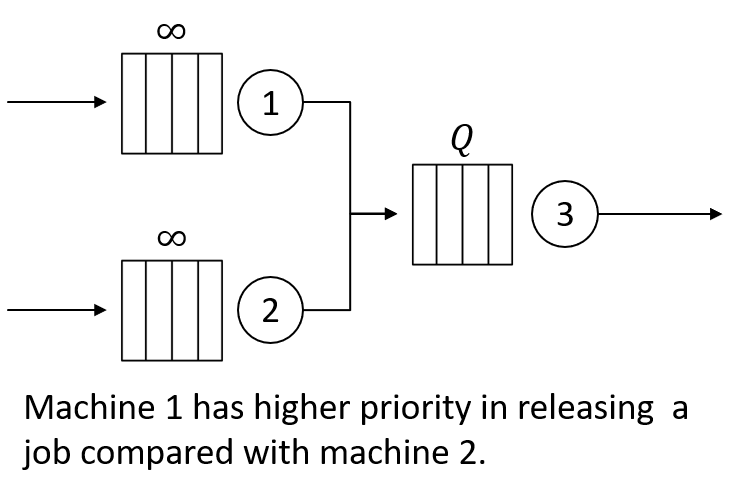
\includegraphics[width=0.4\textwidth]{Figures/merge.png}
	\caption{Example: single server merge.}
	\label{fig:merge}
\end{figure}

State variables have to be defined in the first place, as in Table \ref{tab:merge}. Binary variable $g^{j}$ for $j=1,2,3$ is equal to one if server $j$ is processing a job, otherwise it is equal to zero. Binary variable $b^{j}$ for $j=1,2$ is equal to one if server $j$ is holding a finished job, otherwise it is equal to zero. State variable $b^3$ is not defined, since the job will be released immediately after its processing. Integer variable $q$ represents the number of jobs waiting in buffer 3. 

The events composing the DES model are then defined as in Table \ref{tab:merge}. Event ${(ss,j)}$ for $j=1,2,3$ represents the starting of service of server $j$. If server $j$ is idle, i.e., neither working nor holding a finished part, ${(ss,j)}$ will be scheduled to execute immediately. After an ${(ss,j)}$ is executed, server $j$ becomes active, i.e., state variable $g^j$ is incremented by one. Besides, if server 3 starts a job, the buffer level $q$ is decreased by one. Event ${(d,j)}$ for $j=1,2$ represents the departure of a job from server $j$. A ${(d,1)}$ can be executed if server 1 is holding a finished job and there is at least one space available in buffer 3. A ${(d,2)}$ can be executed immediately if server 2 is holding a finished job, server 1 is not holding a job and there is at least one space available in buffer 3. After executing ${(d,j)}$, the server is not holding any job, hence, state variable $b^{j}$ becomes zero, and the buffer level $q$ is increased by one. Both ${(ss,j)}$ and ${(d,j)}$ can be executed immediately once scheduled, so they are zero-delay. Event ${(sf,j)}$ represents that server $j$ finishes a job, and it is scheduled immediately after ${(ss,j)}$ is executed, and the occurrence delay is equal to the service time, i.e., sampled from $T^{j}$. Thus, ${(ss,j)}$ is a counting event of ${(sf,j)}$. After event ${(sf,j)}$ is executed, server $j$ is no longer working, thus, $g^j$ is decreased by one. Thus, state variable $g^j$ is a counting variable of ${(sf,j)}$, since its value is incremented by one if ${(ss,j)}$ is executed, and decremented by one if  ${(sf,j)}$ is executed. Specially for $j=1,2$, after a job is finished, the server holds a finished job, and state variable $b^j$ is increased by one. %If the simulation run includes $N^1$ jobs from server 1 and $N^2$ jobs from server 2, the number of executions of events $e^{ss,1}$, $e^{f,1}$, $e^{d,1}$ are equal to $N^1$, the number of executions of events $e^{ss,2}$, $e^{f,2}$, $e^{d,2}$ are equal to $N^2$, the number of executions of events $e^{ss,3}$, $e^{f,3}$ are equal to $N^1+N^2$.

\begin{table}[H]
	\begin{tabular}{llllll} 
		\multicolumn{6}{l}{\textbf{State variables}}\\ \hline
		&&&&& Initial\\
		$s$ & \multicolumn{4}{l}{Description}& value\\\hline
		$g^{j}$&\multicolumn{4}{l}{Equal to 1 if server $j$ is working, otherwise equal to 0.}&0\\
		$b^{j}$&\multicolumn{4}{l}{Equal to 1 if server $j$ is blocked, otherwise equal to 0.}&0\\
		$q$&\multicolumn{4}{l}{Number of jobs in the queue.}&0\\
		&&&&&\\
		\multicolumn{6}{l}{\textbf{Zero-delay events}}\\ \hline
		&&&&& State\\
		$\xi$&Description &  \multicolumn{3}{l}{Condition to schedule}& transition\\\hline
		$({ss,1})$ & Start m1 &  \multicolumn{3}{l}{$g^1\le 0\ \&\ b^1\le0 $} & $g^1${\footnotesize++} \\
		$({d,1})$&Depart m1&  \multicolumn{3}{l}{$b^1\ge1\ \&\  q\le Q-1$} &$b^1${\small-}{\small-}, $q${\footnotesize++} \\
		$({ss,2})$& Start m2 &  \multicolumn{3}{l}{$g^2\le 0\ \&\ b^2\le0 $} & $g^2${\footnotesize++} \\
		$({d,2})$&Depart m2&\multicolumn{3}{l}{$b^2\ge1\ \&\ q\le Q-1\ \&\ b^1\le 0$}&  $b^2${\small-}{\small-}, $q${\footnotesize++} \\
		$({ss,3})$ & Start m3 & \multicolumn{3}{l}{$g^3 \le 0\ \&\ q\ge 1$}&$g^3${\footnotesize++}, $q${\small-}{\small-} \\
		&&&&&\\
		\multicolumn{6}{l}{\textbf{Positive-delay events}}\\ \hline
		&&& &  & State \\
		$\xi$&Description & Delay &  Counting event& Counting variable & transition\\\hline
		$({sf,1})$&Finish m1 & $T^{sf,1}$& ${(ss,1)}$&  $g^1$&  $g^1${\small-}{\small-}, $b^1${\footnotesize++}\\	
		$({sf,2})$&Finish m2 & $T^{sf,2}$& ${(ss,2)}$&  $g^2$&  $g^2${\small-}{\small-}, $b^2${\footnotesize++}\\	
		$({sf,3})$&Finish m3 & $T^{sf,3}$& ${(ss,3)}$&  $g^3$&  $g^3${\small-}{\small-}\\	\hline
	\end{tabular}
	\caption{Events to simulate Single-server merge system.}
	\label{tab:merge}
\end{table}

The MPR proposed in this work is as follows.

Group-A, group-C and (B1) (B2) constraints are identical for all systems and all event type as presented in section \ref{sec:const_A},  \ref{sec:const_B} and \ref{sec:const_C2}. 
\begin{eqnarray}
	(A1)-(A7),(B1),(B2),(C1)-(C4) && \forall \xi \in\{(ss,1),(ss,2),(ss,3),(d,1),(d,2)\}\nonumber\\
	&&  \forall\xi \in\{(sf,1),(sf,2),(sf,3)\}\nonumber
\end{eqnarray}

Events $({ss,j})$ for $j=1,2,3$ and $({d,j})$ for $j=1,2$ are all zero-delay, constraints (B3) to (B11) should be applied. Specifically, constraints (B7), (B8), (B10) and (B11) are identical for all systems, and for sake of simplicity, they are not expanded. 
\begin{eqnarray}
	(B7),(B8),(B10),(B11)&& \forall \xi \in\{(ss,1),(ss,2),(ss,3),(d,1),(d,2)\}\nonumber
\end{eqnarray}

Constraints \eqref{merge:ss1,1} and \eqref{merge:ss1,3}, referring to constraints (B4), imply that if an execution of ${(ss,j)}$ is scheduled, machine $j$ is not occupied by a job under processing or finished. Constraints \eqref{merge:ss1,2} and \eqref{merge:ss1,4}, referring to constraints (B6), imply that if variable $v^{ss,j,g^j,1}_k$ or $v^{ss,j,b^j,1}_k$ is equal to one, machine $j$ is occupied by a job under processing or a finished job. Constraints \eqref{merge:ss1,5}, referring to constraints (B9), state that if execution of event ${(ss,1)}$ or ${(ss,2)}$ is not scheduled, it is either because the machine is occupied, or there is already an execution in the future event list. 
\begin{eqnarray}
	%%%%%%%%%%%%%%%%%   \xi=(ss,1)(ss,2)   %%%%%%%%%%%%%%%%%%%%%%%%%%%
	-u^{g^j}_k\ge z^{ss,j}_k-1&& \forall\ j=1,2,k\in \mathbb{K}\label{merge:ss1,1}\\
	u^{g^j}_k\ge v^{ss,j,g^j,1}_k&& \forall\ j=1,2,k\in \mathbb{K}\label{merge:ss1,2}\\
		-u^{b^j}_k\ge z^{ss,j}_k-1&& \forall\ j=1,2,k\in \mathbb{K}\label{merge:ss1,3}
\end{eqnarray}
\begin{eqnarray}
	u^{b^j}_k\ge v^{ss,j,b^j,1}_k&& \forall\ j=1,2,k\in \mathbb{K}\label{merge:ss1,4}\\
	1-z^{ss,j}_k\le v^{ss,j,g^j,1}_k+v^{ss,j,b^j,1}_k+u^{ss,j}_k&& \forall\ j=1,2,k\in \mathbb{K}\label{merge:ss1,5}
\end{eqnarray}

Similarly, constraints \eqref{merge:ss3,1} to \eqref{merge:ss3,5} refer to constraints (B3) to (B6) and (B9) of event ${(ss,3)}$, stating that an execution of event ${(ss,3)}$ can be scheduled if and only if machine 3 is not occupied, there is a job waiting in buffer 3, there is no executions of ${(ss,3)}$ in the future event list. 
\begin{eqnarray}
	%%%%%%%%%%%%%%%%%   \xi=(ss,3)   %%%%%%%%%%%%%%%%%%%%%%%%%%%
	-u^{g^3}_k\ge z^{ss,3}_k-1&& \forall\ k\in \mathbb{K}\label{merge:ss3,1}\\
	u^{g^3}_k\ge v^{ss,3,g^3,1}_k&& \forall\ k\in \mathbb{K}\label{merge:ss3,2}\\
	u^{q}_k\ge z^{ss,3}_k&& \forall\ k\in \mathbb{K}\label{merge:ss3,3}\\
	-u^{q}_k \ge Q(v^{ss,3,q,0}_k-1)&& \forall\ k\in \mathbb{K}\label{merge:ss3,4}\\
	1-z^{ss,3}_k\le v^{ss,3,g^3,1}_k+v^{ss,3,q,0}_k+u^{ss,3}_k&& \forall\ k\in \mathbb{K}\label{merge:ss3,5}
\end{eqnarray}

Constraints \eqref{merge:d1,1} to \eqref{merge:d1,5} refer to constraints (B3) to (B6) and (B9) of event ${(d,1)}$, implying that an execution of event ${(d,1)}$ can be scheduled if and only if there is a finished job in machine 1, there is space available in buffer 3, there is no executions of ${(d,1)}$ in the future event list. 
\begin{eqnarray}
	%%%%%%%%%%%%%%%%%   \xi=(d,1)   %%%%%%%%%%%%%%%%%%%%%%%%%%%
	u^{b^1}_k\ge z^{d,1}_k&& \forall\ k\in \mathbb{K}\label{merge:d1,1}\\
	-u^{b^1}_k\ge v^{d,1,b^1,0}_k-1&& \forall\ k\in \mathbb{K}\label{merge:d1,2}\\
	Q-u^{q}_k\ge z^{d,1}_k&& \forall\ k\in \mathbb{K}\label{merge:d1,3}\\
	u^{q}_k\ge Qv^{d,1,q,1}_k&& \forall\ k\in \mathbb{K}\label{merge:d1,4}\\
	1-z^{d,1}_k\le v^{d,1,b^1,0}_k+v^{d,1,q,1}_k+u^{d,1}_k&& \forall\ k\in \mathbb{K}\label{merge:d1,5}
\end{eqnarray}

Constraints \eqref{merge:d2,1} to \eqref{merge:d2,7} refer to constraints (B3) to (B6) and (B9) of event ${(d,2)}$, depicting that an execution of event ${(d,2)}$ can be scheduled if and only if there is a finished job in machine 2, there is space available in buffer 3, there is no finished job waiting in machine 1, there is no executions of ${(d,2)}$ in the future event list. 
\begin{eqnarray}
	%%%%%%%%%%%%%%%%%   \xi=(d,2)   %%%%%%%%%%%%%%%%%%%%%%%%%%%
	u^{b^2}_k\ge z^{d,2}_k&& \forall\ k\in \mathbb{K}\label{merge:d2,1}\\
	-u^{b^2}_k\ge v^{d,2,b^2,0}_k-1&& \forall\ k\in \mathbb{K}\label{merge:d2,2}\\
	Q-u^{q}_k\ge z^{d,2}_k&& \forall\ k\in \mathbb{K}\label{merge:d2,3}\\
	u^{q}_k\ge Qv^{d,2,q,1}_k&& \forall\ k\in \mathbb{K}\label{merge:d2,4}\\
	-u^{b^1}_k\ge z^{d,2}_k-1&& \forall\ k\in \mathbb{K}\label{merge:d2,5}\\
	u^{b^1}_k\ge v^{d,2,b^1,1}_k&& \forall\ k\in \mathbb{K}\label{merge:d2,6}\\
	1-z^{d,2}_k\le v^{d,2,b^2,0}_k+v^{d,2,q,1}_k+v^{d,2,b^1,1}_k+u^{d,2}_k&& \forall\ k\in \mathbb{K}\label{merge:d2,7}
\end{eqnarray}

Since events ${(sf,j)}$ are positive-delay, constraints (B12) should be applied, as in constraints \eqref{merge:f,1}. A finishing event of machine $j$ can be scheduled after a starting event is executed. 
\begin{eqnarray}
	%%%%%%%%%%%%%%%%%   \xi=(f,j)   %%%%%%%%%%%%%%%%%%%%%%%%%%%
	x^{sf,j}_{i,k} = w^{ss,j}_{i,k} && \forall\ j=1,2,3, i\in \mathbb{I}^{j},k\in \mathbb{K}\label{merge:f,1}
\end{eqnarray}
Constraints \eqref{merge:E_wj} to \eqref{merge:E_q} indicate the evolution of state variables $g^j$, $b^j$ and $q$, respectively. $g^j$ is increased by one if machine $j$ starts a job and decreased by one if it finished a job. $b^j$ is increased by one if machine $j$ finishes a job, and decreased by one if it releases a job. $q$ is increased by one if machine 1 or 2 releases a job, and decreased by one if machine 3 seizes a job from buffer 3. The rest of the model indicates the initialization and range of state variables.
\begin{eqnarray}
	%%%%%%%%%%%%%%%%%   constraints E  %%%%%%%%%%%%%%%%%%%%%%%%%%% 
	u^{g^j}_k=u^{g^j}_{k-1}+ \sum_{i\in\mathbb{I}^j}w^{ss,j}_{i,k}-\sum_{i\in\mathbb{I}^j}w^{sf,j}_{i,k}&& \forall\ j=1,2,3, k\in \mathbb{K}\label{merge:E_wj}\\
	u^{b^j}_k=u^{b^j}_{k-1}+ \sum_{i\in\mathbb{I}^j}w^{sf,j}_{i,k}-\sum_{i\in\mathbb{I}^j}w^{d,j}_{i,k}&& \forall\ j=1,2, k\in \mathbb{K}\label{merge:E_bj}\\
	u^{q}_k=u^{q}_{k-1}+\sum_{j=1,2}\sum_{i\in\mathbb{I}^j}w^{d,j}_{i,k}-\sum_{i\in\mathbb{I}^3}w^{ss,3}_{i,k}&& \forall\ k\in \mathbb{K}\label{merge:E_q}\\
	u^{g^1}_0=u^{g^2}_0=u^{g^3}_0=u^{b^1}_0=u^{b^2}_0=u^{q}_0=0\nonumber\\
	u^{g^1}_{k},u^{g^2}_{k},u^{g^3}_{k},u^{b^1}_{k},u^{b^2}_{k}\in\{0,1\},\ u^q_{k}\in\{0,...,Q\}&& \forall\ k\in \mathbb{K}\nonumber
\end{eqnarray}




\subsection{G/G/1 with failure}
A G/G/1 queueing system with unreliable server is studied in this section. The server has two states, up and down, respectively. When the server is in up state, it can process a job. When the server turns to down state from up state, the repair starts immediately, and if the server is processing a job, the job is discarded. After the repair finishes, the server turns to up state, and restarts to process new jobs. The repair time follows a general distribution. The server will then keep in up state for a certain time called \textit{up time}, following a general distribution, and will fail again. The failure is time-dependent. Jobs arrive at the system following a general arrival process and enter the queue in front of the server. When the server is in up state and idle, the server can take a job from the queue and start the service. After the service, a job can be immediately released from the system.

As in Table \ref{tab:failure}, the state variables include integer variable $q$ representing the number of jobs in the queue, binary variable $g$ indicating whether the server is working or not, binary variable $h$ indicating whether the server is in down state or not.%, and binary variable $r$ representing whether the server is under repair.

The events composing the DES model are then defined as in Table \ref{tab:failure}. Event ${arr}$ indicates that a job arrives at the system, and it is scheduled after a previous arrival, with a delay equal to the inter-arrival time. A counting event of ${arr}$, i.e., ${\tilde{arr}}$, and a counting variable $u^{arr}$ should be defined. The condition to schedule an arrival is that there is no execution of ${arr}$ in the future event list. When ${\tilde{arr}}$ is executed, the counting variable $u^{arr}$, i.e., the number of executions of ${arr}$ in the future event list, will be increased by one. When ${arr}$ is executed, the number of jobs in the queue will be increased by one, and the counting variable $u^{arr}$ will be decreased by one. Event ${ss}$ represents that the server starts to process a job. If and only if there is at least one job in the queue, the server is in up state and idle, event ${ss}$ is scheduled. When event ${ss}$ is executed, the number of jobs in the queue is reduced by one, and the server starts to work, i.e., state variable $g$ becomes one. Event ${sf}$ represents that a server finishes a job, and one execution of it is scheduled each time a job is started, and the occurrence delay is equal to the service time of the job. Event ${ss}$ is the counting event, and state variable $g$ is the counting variable of ${sf}$. After ${sf}$ is executed, the server becomes idle. Once the server is in down state, job under process is discarded, i.e., scheduled execution of ${sf}$ is canceled. Event ${fl}$ represents that the state of the server becomes down, and it is scheduled after the previous repair finishes with delay equal to the up time. Since it is positive-delay, a counting event ${\tilde{fl}}$ should be added, and also a counting variable $u^{fl}$. The condition to schedule an ${\tilde{fl}}$ is that the server is in up state, i.e., $h$ equal to zero, and there is no execution of ${fl}$ in the future event list, i.e., $u^{fl}$ smaller than or equal to zero. When ${\tilde{fl}}$ is executed, the number of executions of ${fl}$ is increased by one. When ${fl}$ is executed, the server is in down state, it cannot be working, i.e., $g$ equal to zero, and its number of executions in the future event list is reduced by one. Event ${srp}$ represents start of repair, and it is scheduled if the server is in down state and not under repair, and executed with no delay. When it is executed, the server is under repair. Event ${frp}$ states the finish of repair, and it is scheduled after event ${srp}$ is executed, hence, ${srp}$ is the counting event, and state variable $u^{frp}$ is introduced as the counting variable. After it is executed, the server becomes up, and no longer under repair. %If the simulation included $N$ arrivals and $N^{fl}$ failures, the number of executions of $e^{\tilde{arr}}$, $e^{ss}$, $e^{arr}$ and $e^{f}$ is equal to $N$, and the number of executions of $e^{\tilde{fl}}$, $e^{srp}$, $e^{fl}$ and $e^{frp}$ is equal to $N^{fl}$.

\begin{table}[H]
	\begin{tabular}{lllllll} 
		\multicolumn{7}{l}{\textbf{State variables}}\\ \hline
		&&&&&& Initial\\
		$s$ & \multicolumn{5}{l}{Description}& value\\\hline
		$g$&\multicolumn{5}{l}{Equal to 1 if server is working on a job, otherwise equal to 0.}&0\\
		$h$&\multicolumn{5}{l}{Equal to 1 if server fails, otherwise equal to 0.}&0\\
		$q$&\multicolumn{5}{l}{Number of jobs in the queue.}&0\\
		$u^{frp}$&\multicolumn{5}{l}{Number of executions with event type $frp$ in the future event list.}&0\\
		$u^{arr}$&\multicolumn{5}{l}{Number of executions with event type $arr$ in the future event list.}&0\\
		$u^{fl}$&\multicolumn{5}{l}{Number of executions with event type $fl$ in the future event list.}&0\\
		&&&&&&\\
		\multicolumn{7}{l}{\textbf{Zero-delay events}}\\ \hline
		&&&&& State&\\
		$\xi$&Description &  \multicolumn{3}{l}{Condition to schedule}& transition&\\\hline
		${\tilde{arr}}$ & Counting arrival &  \multicolumn{3}{l}{$u^{arr}\le 0$} & $u^{arr}${\footnotesize++}& \\
		${ss}$&Start&  \multicolumn{3}{l}{$1\le q,\ g\le 0,\ h\le 0$} &$g${\footnotesize++}, $q${\small-}{\small-}&  \\
		${\tilde{fl}}$& Counting failure &  \multicolumn{3}{l}{$h\le 0,\ u^{fl}\le 0$} & $u^{fl}${\footnotesize++}& \\
		${srp}$&Start to repair&\multicolumn{3}{l}{$h\ge 1,\ u^{frp}\le 0$}&  $u^{frp}${\footnotesize++}&  \\
		&&&&&&\\
		\multicolumn{7}{l}{\textbf{Positive-delay events}}\\ \hline
		&&& Counting& Counting  & State& Condition\\
		$\xi$&Description & Delay &  event& variable & transition&to cancel\\\hline
		${arr}$&Arrival & $T^{arr}$& ${\tilde{arr}}$&  $u^{arr}$&  $u^{arr}${\small-}{\small-},  $q${\footnotesize++}&\\	
		${sf}$&Finish & $T^{sf}$& ${ss}$&  $g$&  $g${\small-}{\small-}&$h\ge 1$, $g\ge 1$\\	
		${fl}$&Failure & $T^{fl}$& ${\tilde{fl}}$&  $u^{fl}$&   $h${\footnotesize++}, $u^{fl}${\small-}{\small-}&\\	
		${frp}$&Finish of repair & $T^{rp}$& ${srp}$&  $u^{frp}$&   $h${\small-}{\small-}, $u^{frp}${\small-}{\small-}&\\	\hline
	\end{tabular}
	\caption{Events to simulate G/G/1 with failure.}
	\label{tab:failure}
\end{table}

The MPR proposed in this work is as follows.

Constraints (A1)-(A7), (C1)-(C4) and (B1) (B2) are applied to all events. Events ${\tilde{arr}}$, ${ss}$, ${\tilde{fl}}$ and ${srp}$ are all zero-delay, constraints (B3) to (B11) should be applied, and constraints (B12) should be applied to events ${arr}$, ${sf}$, ${fl}$ and ${frp}$. Those constraints have been explained in the previous two examples, and then this example will not expand them. 


\begin{eqnarray}
	(A1)-(A7),(B1),(B2),(C1)-(C4)&& \forall \xi \in\{\tilde{arr},ss,\tilde{fl},srp\}\nonumber\\
	&&  \forall\xi \in\{arr,sf,fl,frp\}\nonumber\\
	(B3)-(B11)&& \forall \xi \in\{\tilde{arr},ss,\tilde{fl},srp\}\nonumber\\
	(B12)&& \forall\xi \in\{arr,sf,fl,frp\}\nonumber
\end{eqnarray}

Constraints \eqref{fail:D1} to \eqref{fail:D14} are group-D constraints for canceling event ${sf}$. Binary variable $z^{\bar{sf}}_k$ is equal to one if executions of ${sf}$ are removed from the future event list, otherwise the execution is not canceled. Specifically, constraints \eqref{fail:D1} and \eqref{fail:D3} show that if ${sf}$ is canceled, state variable $h$ must be greater than or equal to one, and there is at least one execution of $sf$ in the future event list. Constraints \eqref{fail:D2} indicate that if $v^{\bar{sf},h,0}$ is equal to one, the machine is in up state. Constraints \eqref{fail:D4} indicate that if $v^{\bar{sf},g,0}$ is equal to one, there is no executions of ${sf}$ in the future event list. Constraints \eqref{fail:D5} show that if executions of ${sf}$ are not canceled, i.e., $z^{\bar{sf}}_k$ is equal to zero, either the machine in in up state or there is no execution in the event list. 
\begin{eqnarray}
	u^{h}_k\ge z^{\bar{sf}}_k&&\forall\ k\in \mathbb{K}\label{fail:D1}\\
	-u^{h}_k\ge v^{\bar{sf},h,0}_k-1&&\forall\ k\in \mathbb{K}\label{fail:D2}\\
	u^{g}_{k-1}\ge z^{\bar{sf}}_k &&\forall\ k\in \mathbb{K}\label{fail:D3}\\
	-u^{g}_{k-1} \ge v^{\bar{sf},g,0}_k-1&&\forall\ k\in \mathbb{K}\label{fail:D4}\\
	1-z^{\bar{sf}}_k\le v^{\bar{sf},s,0}_k+v^{\bar{sf},g,0}_k&&\forall\ k\in \mathbb{K}\label{fail:D5}
\end{eqnarray}

Integer variables $k^{sf,0}_i$ and $k^{sf,1}_{i}$ denote the iteration index when the $i$-th execution of ${sf}$ is scheduled and executed, as in constraints \eqref{fail:D6} and \eqref{fail:D7}. 
\begin{eqnarray}
	k^{f,1}_i=\sum_{k\in\mathbb{K}}kw^{sf}_{k,i}&&\forall\ i\in \mathbb{I}^{\xi}\label{fail:D6}\\
	k^{f,0}_i=\sum_{k\in\mathbb{K}}kx^{sf}_{k,i}&&\forall\ i\in \mathbb{I}^{\xi}\label{fail:D7}
\end{eqnarray}
Binary variable $\theta^{sf}_{i,k}$ equal to one represents that $i$-th execution of event ${sf}$ is canceled in iteration $k$. Constraints \eqref{fail:D8} and \eqref{fail:D9} state that if the $i$-th execution of ${sf}$ is canceled in iteration $k$, then it must be scheduled before iteration $k$ and executed after iteration $k$. Binary variable $\phi^{sf,0}_{i,k}$ equal to one indicates that the condition to cancel ${sf}$ is not true in iteration $k$ or the $i$-th execution of ${sf}$ is scheduled after iteration $k$, as in constraints \eqref{fail:D10}. Binary variable $\phi^{sf,1}_{i,k}$ equal to one indicates that the $i$-th execution of ${sf}$ is executed before iteration $k$, as in constraints \eqref{fail:D11}. Constraints \eqref{fail:D12} state that if execution $i$ of ${sf}$ is not canceled in iteration $k$, it is either because the condition to cancel is false, or it is executed before or scheduled after iteration $k$. 
\begin{eqnarray}
	kz^{\bar{sf}}_k -k^{sf,0}_i - 1 \ge K(\theta^{sf}_{i,k}-1)&&\forall\ i\in \mathbb{I}^{\xi},k\in \mathbb{K}\label{fail:D8}\\
	k^{sf,1}_i - 1 - kz^{\bar{sf}}_k \ge k(\theta^{sf}_{i,k}-1)&&\forall\  i\in \mathbb{I}^{\xi},k\in \mathbb{K}\label{fail:D9}\\
	k^{sf,0}_i - kz^{\bar{sf}}_k \ge k(\phi^{sf,0}_{i,k}-1)&&\forall\ i\in \mathbb{I}^{\xi},k\in \mathbb{K}\label{fail:D10}
\end{eqnarray}
\begin{eqnarray}
	kz^{\bar{sf}}_k - k^{sf,1}_i \ge K(\phi^{sf,1}_{i,k}-1)&&\forall\ i\in \mathbb{I}^{\xi},k\in \mathbb{K}\label{fail:D11}\\
	1-\theta^{sf}_{i,k} \le \phi^{sf,0}_{i,k} + \phi^{sf,1}_{i,k}&&\forall\ i\in \mathbb{I}^{\xi},k\in \mathbb{K}\label{fail:D12}
\end{eqnarray}

Binary variable $\gamma^{sf}_{i,k}$ equal to one represents that the $i$-th execution of event $sf$ is performed in iteration $k$, and it is not canceled, as in constraints \eqref{fail:D14}. Constraints \eqref{fail:D13} state that if $\gamma^{sf}_{i,k}$ is equal to zero, it is either because the execution is not performed in iteration $k$ or it is canceled. 
\begin{eqnarray}
	\gamma^{sf}_{i,k} \ge w^{sf}_{i,k} - \sum_{k^{'}\in \mathbb{K}}\theta^{sf}_{i,k^{'}}&&\forall\ i\in \mathbb{I}^{\xi},k\in \mathbb{K}\label{fail:D13}\\
	w^{sf}_{i,k} - \sum_{k^{'}\in \mathbb{K}}\theta^{sf}_{i,k^{'}} -1 \ge (N^{fl}+1)(\gamma^{sf}_{i,k}-1) &&\forall\ i\in \mathbb{I}^{\xi},k\in \mathbb{K}\label{fail:D14}
\end{eqnarray}

Constraints \eqref{fail:E1} to \eqref{fail:E7} depict the evolution of state variables. Constraints \eqref{fail:E1} to \eqref{fail:E4}, referring to constraints (E5) and (E6), are similar to the two examples previously discussed, state variables $u^{arr}$, $q$, $u^{fl}$ and $u^{frp}$ are all changed by events without cancellation. Constraints \eqref{fail:E5} state that if event ${sf}$ is canceled in iteration $k$, the number of executions of ${sf}$ in the future event list will be reduced to zero. Constraints \eqref{fail:E6} and \eqref{fail:E7} show that if ${sf}$ is not canceled in iteration $k$, the state variable $g$ will be increased by one if ${ss}$ is executed, and decreased by one if ${sf}$ is executed without being canceled. The rest of the model indicates the initialization and range of state variables.
\begin{eqnarray}
	u^{arr}_k=u^{arr}_{k-1}+ \sum_{i\in\mathbb{I}^j}w^{\tilde{arr}}_{i,k}-\sum_{i\in\mathbb{I}^j}w^{arr}_{i,k}&&\forall\ k\in \mathbb{K}\label{fail:E1}\\
	u^{q}_k=u^{q}_{k-1}+ \sum_{i\in\mathbb{I}^j}w^{arr}_{i,k}-\sum_{i\in\mathbb{I}^j}w^{ss}_{i,k}&&\forall\ k\in \mathbb{K}\label{fail:E2}\\
	u^{fl}_k=u^{fl}_{k-1}+ \sum_{i\in\mathbb{I}^j}w^{\tilde{fl}}_{i,k}-\sum_{i\in\mathbb{I}^j}w^{fl}_{i,k}&&\forall\ k\in \mathbb{K}\label{fail:E3}\\
	u^{frp}_k=u^{frp}_{k-1}+ \sum_{i\in\mathbb{I}^j}w^{srp}_{i,k}-\sum_{i\in\mathbb{I}^j}w^{frp}_{i,k}&&\forall\ k\in \mathbb{K}\label{fail:E4}\\
	u^{g}_k \le 1-z^{\bar{sf}}_{k}&&\forall\ k\in \mathbb{K}\label{fail:E5}\\
	u^{g}_k\le u^{g}_{k-1}- \sum_{i\in \mathbb{I}} \gamma^{sf}_{i,k} +\sum_{i\in \mathbb{I}} w^{ss}_{i,k} + z^{\bar{sf}}_{k}&&\forall\ k\in \mathbb{K}\label{fail:E6}\\
	u^{g}_k\ge u^{g}_{k-1}-  \sum_{i\in \mathbb{I}} \gamma^{sf}_{i,k} +\sum_{i\in \mathbb{I}} w^{ss}_{i,k}  - z^{\bar{sf}}_{k}&&\forall\ k\in \mathbb{K}\label{fail:E7}\\
	u^{arr}_0=u^{fl}_0=u^{r}_0=u^{g}_0=u^{q}_0=0\nonumber\\
	u^{arr}_k,u^{fl}_k,u^{frp}_k,u^{g}_k\in\{0,1\},\ u^{q}_k\in\{0,...,Q\}\nonumber
\end{eqnarray}

\bigskip
Given the set of state variables, the set of zero-delay events, the sets of positive-delay events, as in Tables \ref{tab:ggm_1}, \ref{tab:merge}, \ref{tab:failure}, and also $K$ and $N^{\xi}$, the total number of  iterations and the maximum number of executions of each event, respectively, the implementation of the proposed approach is trivial. Appendix I provides the pseudo code of the proposed approach. As it can be seen, the algorithm is composed of several for-loops only. The java source code of an automatic MPR generation procedure can be found on the repository at https://github.com/myrazhang/MPRofDES.

\section{Discussion}\label{sec:discussion}

The MPR proposed in this work differs from the state-of-the-art MPR (\cite{chan2008optimization}) in the objective function. In the state-of-the-art formulation, the constraints represent the event triggering relationships, i.e., the execution time of the triggered event must be later than that of the triggering event with an occurrence delay. Hence, the objective function must be the minimization of the execution time of all the events, so that all the events are executed as soon as possible. In this work, the constraints represent that once the condition to schedule or cancel an event is true, the event must be scheduled or canceled, i.e., the logic that events must be executed as soon as possible is forced by constraints. Thus, the objective function can be defined in a more flexible way. 

The proposed MPR presents only the realization of a sample path of DES, since it takes the samples of random variates as the coefficients of constraints. However, expanding the MPR from single-sample-path model into a multiple-sample-path model can be achieved by adding one more subscript to each decision variables, for instance, $\mathcal{E}_k$ replaced by $\mathcal{E}_{k,r}$ where $r$ represents $r$-th replicates. The resulting MPR is separable since there are not constraints linking variables from different sample paths, i.e., the sample paths are independent from each other. Multiple-sample-path models can be plugged into retrospective algorithms so that optimization problems considering sampling noise can be solved.

As it can be seen, the proposed MPR contains both integer variables and real-valued variables. Furthermore, if the steady state performance from simulation model is of interest, the simulation length, i.e., the number of event executions, is usually long. Thus, the MPR has many variables and constraints. For instance, the MPR of G/G/m model with simulation length equal to $1000$ jobs contains 12,000 real-valued and more than 32,000,000 integer variables and more than 64,000,000 constraints. It is more reasonable to use the MPR as a white-box representation of DES, other than solving it with an optimizer because the computational complexity is extremely high. 

An application of the MPR is the calculation of gradient/sub-gradient from a simulation run, based on the sensitivity analysis of an approximate linear programming (LP) of the MPR. The procedure is as follows. The DES is first simulated with an event-scheduling execution logic, and the optimal solution of the MPR can be obtained during the simulation run. The approximate LP is formulated by replacing all the decision variables with a big-M multiplier, i.e., all variables except the ones representing event scheduling times, execution times, and state variables, with the value in the optimal solution, and relaxing the integrality of the remaining variables. By solving the dual problem of the approximate LP, an approximate gradient/sub-gradient of the objective function can be obtained on some coefficients (for instance, parameters of the distribution of occurrence delay $T^{\xi}$, or the thresholds $a^{\xi,s}$ and $c^{\xi,s}$ of the ranges that compose the conditions to schedule or cancel events, which are part of the conditions to schedule events). Under the black-box settings, deriving the gradient/sub-gradient must exploiting the neighborhood with several simulation runs, and the number of simulation runs needed to get the gradient of one point grows exponentially on the dimension, thus the proposed white-box MPR of DES can save the computational time for simulation.

Another way to make use of the MPR is to derive an MPR of a simulation optimization problem, as previously introduce while discussing objective function flexibility. In the applications in manufacturing and service operations, the decision variables of an optimization problem are usually the thresholds $a^{\xi,s}$ and $c^{\xi,s}$ of the ranges that compose the conditions to schedule or cancel events, which are part of the conditions to schedule events. So, to transform the MPR of simulation into MPR of simulation optimization, one just needs to specify that certain thresholds are decision variables instead of coefficients. Then, the system performance could be in the objective function or in a constraint stating that it must achieve a target. The convenience of transforming the proposed MPR into an MPR of simulation optimization represents another contribution of this work, and simulation-based optimization techniques enriched with the MPR can be developed in the future.

%However, the resulting MPR still has computational issue, which leads to our future research interest.


\section{Conclusion}\label{sec:conclusion}

This work proposes an MPR of a sample path of a DES model that satisfies certain assumptions, based on the widely applied event-scheduling execution logic of DES. In the MPR, the decision variables include event scheduling times, execution times, and system state after each event execution, and the constraints represent that events are scheduled or canceled when the system state satisfies the condition to schedule or cancel. Furthermore, the MPR also takes the samples of random variates as the coefficients of constraints, where the random variates are usually the time delay between the occurring time and scheduling time of an event execution. The equivalence of the MPR and the simulation run implemented with an event-scheduling algorithm has been validated using several cases. 

The proposed approach enriches the DES with an equivalent white-box MPR. In the literature, most of the simulation-based optimization techniques consider DES as black-box, which usually requires intensive simulation budget. Based on this work, it will be possible to develop optimization techniques taking advantage of the white-box representation. Future work will be dedicated to developing such research direction, such as efficient gradient/sub-gradient generation algorithms or optimization approaches to solve design or operation problems in manufacturing and service systems, for instance finding the optimal capacities of the queues or the control policy. 

%Reference
\bibliographystyle{apacite}
\bibliography{RAP, Biblio_Loop}

\section*{Appendix I: implementation pseudo code}
The pseudo code below shows the implementation of the proposed approach. The algorithm requires $\mathbb{X}$, $\textbf{s}_0$, $\mathbb{S}^{\xi}$, $\mathbb{S}^{\bar{\xi}}$, $\mathbb{S}^{c}$, $K$ and $N^{\xi}$ as the input. In the main implementation of the algorithm, each constraint introduced in Section 2.4 is written inside certain for-loop. The expression of the constraints depends on the grammar of the state-of-the-art optimizer one want to use, such as Cplex, Gurobi, etc.

\begin{breakablealgorithm}
	\label{algo:implement_MPR}
	\caption{Implementation pseudo code.}
	\begin{algorithmic}[1]
		\REQUIRE ~~\\
		$\mathbb{X}$: set of events.\\
		$\textbf{s}_0$: initial system state.\\
		$\mathbb{S}^{\xi}$: set of state variables included in the condition to schedule event $\xi$.\\
		$\mathbb{S}^{\bar{\xi}}$: set of state variables included in the condition to cancel event $\xi$.\\
		$\mathbb{S}^{c}$: set of counting variable.\\
		$K$: number of iterations until the termination of simulation. \\
		$N^{\xi}$: execution number of event $\xi$.
		\STATE (A6) (E7)
		\FOR {$\xi\in\mathbb{X}$ }
		\FOR{$i=1\ to\ N^{\xi}$}
		\FOR {$k=1\ to\ K$}
		\STATE (A1) (A2) (B1) (B2)
		\ENDFOR
		\STATE (A3) (A7) (C2) (C3)
		\ENDFOR
		\FOR{$i=1\ to\ N^{\xi}-1$}
		\STATE (C1) (C4)
		\ENDFOR	
		\ENDFOR
		
		\FOR {$k=1\ to\ K$}
		\STATE (A4) (A5)
		\ENDFOR
		
		\FOR {each zero-delay event $\xi\in\mathbb{X}$}
		\FOR {$k=0\ to\ K-1$}
		\FOR {$s\in\mathbb{S}^{\xi}$}
		\STATE (B3) (B4) (B5) (B6)
		\ENDFOR
		\STATE (B7) (B9) (B10)
		\ENDFOR
		\STATE (B8)
		\FOR{$i=1\ to\ N^{\xi}$}
		\STATE (B11)
		\ENDFOR	
		\ENDFOR
		
		\FOR {each positive-delay event $\xi\in\mathbb{X}$}
		\FOR {$k=0\ to\ K-1$}
		\FOR{$i=1\ to\ N^{\xi}$}
		\STATE (B12) (D6) (D7) (D8) (D9) (D10) (D11) (D12) (D13) (D14)
		\ENDFOR	
		\FOR{$s\in\mathbb{S}^{\bar{\xi}}$}
		\STATE (D1) (D2) (D3) (D4)
		\ENDFOR	
		\STATE (D5)
		\ENDFOR	
		\ENDFOR
		
		\FOR {$k=0\ to\ K-1$}
		\FOR {$s\in\mathbb{S}/\mathbb{S}^c$}
		\STATE (E1)
		\ENDFOR
		\FOR {$s\in\mathbb{S}^c$}
		\STATE (E2) (E3) (E4)
		\ENDFOR
		\ENDFOR
		
	\end{algorithmic}
\end{breakablealgorithm}


\section*{Appendix II: Event-scheduling algorithm}

\begin{breakablealgorithm}
	\label{algo:DES}
	\caption{Event-scheduling algorithm.}
	\begin{algorithmic}[1]
		\REQUIRE ~~\\
		Set of events $\mathbb{X}$.\\
		Initial system state: $\textbf{s}_0$.\\
		Simulation length: number of iterations $K$. \\
		Simulation clock: \textit{clock} = 0.\\
		Number of scheduled executions of event type $\xi$: $i^{\xi}=0$.\\
		\textit{FutureEventList} = \{\}.\\
		
		
		\FOR {k=0 to K-1}
		\STATE \textbf{Schedule new executions}
		\FOR{each event $\xi\in\mathbb{X}$}
		\IF{$CS^{\xi}(\textbf{s}_{k})$}
		\STATE $i^{\xi} = i^{\xi}+1$
		\STATE Sample occurring delay $t^{\xi}_{i^{\xi}}$ from random variate $T^{\xi}$
		\STATE Add execution $(\xi,i^{\xi},clock,clock+t^{\xi}_{i^{\xi}})$ to \textit{FutureEventList}.
		\ENDIF
		\ENDFOR
		\STATE
		
		\STATE \textbf{Cancel executions}
		\FOR {each execution \textit{exe}$\in$\textit{FutureEventList}}
		\IF {$CC^{exe.event\_type}(\textbf{s}_{k})$}
		\STATE Remove \textit{exe} from \textit{FutureEventList}
		\ENDIF
		\ENDFOR
		
		\STATE
		\STATE \textbf{Perform the earliest execution}
		\STATE From \textit{FutureEventList}, take execution $exe$, which is with the earliest occurring time. 
		\STATE Update system state: $\textbf{s}_{k+1}\leftarrow F^{exe.event\_type}(\textbf{s}_{k})$.
		\STATE $clock$ = $exe.occurring\_time$.
		
		\ENDFOR
	\end{algorithmic}
\end{breakablealgorithm}


\section*{Appendix III: Modified event-scheduling logic.}

\begin{breakablealgorithm}
	\label{algo:modified_DES}
	\caption{Modified event-scheduling logic.}
	\begin{algorithmic}[1]
		\FOR {k=0 to K-1}
		\STATE \textbf{Schedule new zero-delay executions}
		\FOR{each zero-delay event $\xi\in\mathbb{X}$}
		\IF{$CS^{\xi}(\textbf{s}_{k})$ \& there is no execution of event $\xi$ in \textit{FutureEventList}}
		\STATE $i^{\xi} = i^{\xi}+1$
		\STATE Add execution $(\xi,i^{\xi},$clock$,$clock$,false)$ to \textit{FutureEventList}.
		\ENDIF
		\ENDFOR
		\STATE
		
		\STATE \textbf{Cancel executions}
		\FOR {each positive-delay execution \textit{exe}$\in$\textit{FutureEventList}}
		\IF {$CC^{\xi}(\textbf{s}_{k})$}
		\STATE \textit{exe.cancel} = true, $u^{\xi}=0$.
		\ENDIF
		\ENDFOR
		
		\STATE
		\STATE \textbf{Perform an execution}
		\STATE From \textit{FutureEventList}, take execution $exe$, which is with the earliest occurring time. 
		\STATE $clock$ = $exe.occurring\_time$.
		\IF{$T^{\xi}>0$}
		\IF{$exe.cancel$ is false}
		\STATE Update system state: $\textbf{s}_{k+1}\leftarrow F^{\xi}(\textbf{s}_{k})$.
		\ENDIF
		\ELSE
		\STATE Update system state: $\textbf{s}_{k+1}\leftarrow F^{\xi}(\textbf{s}_{k})$.
		\STATE \textbf{Schedule new positive-delay execution}
		\IF{$\xi$ is the counting event of $\xi^{'}$}
		\STATE Sample $t^{\xi^{'}}_{i}$ from random variate $T^{\xi^{'}}$.
		\STATE Add execution $(\xi^{'},i,$clock$,$clock$+t^{\xi^{'}}_{i},false)$ to \textit{FutureEventList}.
		\ENDIF		
		\ENDIF
		%\STATE \textbf{Schedule new positive-delay executions}
		
		\ENDFOR
	\end{algorithmic}
\end{breakablealgorithm}


%\end{multicols}

\end{document}
